\chapter{Corpus linguistics as a scientific method}
\label{ch:scientificmethod}

At the end of the previous chapter, we defined corpus linguistics as ``the investigation of linguistic research questions that have been framed in terms of the conditional distribution \is{distribution!conditional} of linguistic phenomena in a linguistic corpus'' and briefly discussed the individual steps necessary to conduct research on the basis of this discussion.

In this chapter, we will look in more detail at the logic and practice of formulating and testing research questions (Sections \ref{sec:statinghypotheses} and \ref{sec:testinghypotheses}). We will then discuss the notion of operationalization \is{operationalization} in some detail (Section~\ref{sec:operationalization}) before closing with some general remarks about the place of hypothesis \is{hypothesis} testing in scientific research practice (Section~\ref{sec:researchcycle}).

\section{The scientific hypothesis}
\label{sec:scientifichypothesis}

Broadly speaking, there are two ways in which we can state our research question: first, in the form of an actual \emph{question} such as ``Is there a relationship between X and Y?'' or ``What is the relationship between X and Y?''; second, in the form of a specific \emph{hypothesis} \is{hypothesis} concerning the relationship between two variables, such as ``all X are Y'' or ``X leads to Y''.

The first way entails a relatively open\hyp{}minded approach to our data. We might have some general expectation of what we will find, but we would put them aside and simply start collecting observations \is{observational method} and look for patterns. If we find such patterns, we might use them to propose a provisional generalization, which we successively confirm, modify or replace on the basis of additional observations until we are satisfied that we have found the broadest generalization that our data will allow -- this will then be the answer to our research question.

This so\hyp{}called \emph{inductive} \is{induction} approach was famously rejected by the Austrian-Brit\-ish philosopher \ia{Popper, Karl R.@Popper, Karl R.}Karl Popper for reasons that will become clear below, but after a period of disrepute it has been making a strong comeback in many disciplines in recent years due to the increasing availability of massive amounts of data and of tools that can search for correlations \is{correlation} in these data within a reasonable time frame (think of the current buzz word ``big data''). Such massive amounts of data allow us to take an extremely inductive \is{induction} approach -- essentially just asking ``What relationships exist in my data?'' -- and still arrive at reliable \is{reliability} generalizations. Of course, matters are somewhat more complex, since, as discussed at the end of the previous chapter, theoretical constructs cannot directly be read off our data. But the fact remains that, used in the right way, inductive \is{induction} research designs \is{research design} have their applications. In corpus linguistics, large \is{corpus size} amounts of data have been available for some time (as mentioned in the previous chapter, the size even of corpora striving for some kind of balance is approaching half\hyp{}a-billion words), and inductive approaches are used routinely and with insightful consequences (\citealt{sinclair_corpus_1991} is an excellent example).

The second way of stating research questions entails a more focused way of approaching our data. We state our hypothesis \is{hypothesis} before looking at any data, and then limit our observations \is{observational method} just to those that will help us determine the truth of this hypothesis (which is far from trivial, as we will see presently). This so\hyp{}called \emph{deductive} \is{deduction} approach is generally seen as the standard way of conducting research (at least ideally -- actual research by actual people tends to be a bit messier even conceptually).

We will generally take a deductive \is{deduction} approach in this book, but it will frequently include inductive (exploratory) excursions, as induction \is{induction} is a often useful in itself (for example, in situations where we do not know enough to state a useful working hypothesis \is{hypothesis} or where our aim is mainly descriptive) \is{description} or in the context of deductive research (where a first exploratory \is{exploration} phase might involve inductive \is{induction} research as a way of generating hypotheses). We will see elements of inductive research in some of the case studies in Part II of this book.

\subsection{Stating hypotheses}
\label{sec:statinghypotheses}

As indicated above, scientific hypotheses are typically statements relating two variables, but in order to understand what makes such statements special, let us take a step back and look at the simpler statement in (\ref{ex:englishhaswindscreen}):

\begin{exe}
\ex The English language has a word for the forward\hyp{}facing window of a car.
\label{ex:englishhaswindscreen}
\end{exe}

Let us assume, for the moment, that we agree on the existence of something called \textit{car} that has something accurately and unambiguously described by `forward\hyp{}facing window', and that we agree on the meaning \is{semantics} of ``English'' and ``language X has a word for Y''. How could we prove the statement in (\ref{ex:englishhaswindscreen}) to be true? There is only one way: we have to find the word in question. We could, for example, describe the concept \textvv{Forward\hyp{}Facing Window of Car} to a native speaker or show them a picture of one, and ask them what it is called (a method used in traditional dialectology and field linguistics). Or we could search a corpus for all passages mentioning cars and hope that one of them mentions the forward\hyp{}facing window; alternatively, we could search for grammatical contexts in which we might expect the word to be used, such as $\langle$ \texttt{through the NOUN of POSS.PRON car} $\rangle$ (see Section~\ref{sec:retrieval} in \chapref{ch:retrievalannotation} on how such a query \is{query} would have to be constructed). Or we could check whether other people have already found the word, for example by searching the definitions of an electronic dictionary. \is{dictionary} If we find a word referring to the forward\hyp{}facing window of a car, we have thereby proven its existence -- we have \emph{verified} the statement in (\ref{ex:englishhaswindscreen}).

But how could we \emph{falsify} \is{falsification} the statment, i.e., how could we prove that English does \emph{not} have a word for the forward\hyp{}facing window of a car? The answer is simple: we can't. As discussed extensively in \chapref{ch:needforcorpus}, both native\hyp{}speaker knowledge and corpora are necessarily finite. Thus, if we ask a speaker to tell us what the forward\hyp{}facing window of car is called and they don't know, this may be because there is no such word, or because they do not know this word (for example, because they are deeply uninterested in cars). If we do not find a word in our corpus, this may be because there is no such word in English, or because the word just happens to be absent from our corpus, or because it does occur in the corpus but we missed it. If we do not find a word in our dictionary, \is{dictionary} this may be because there is no such word, or because the dictionary\hyp{}makers \is{dictionary} failed to include it, or because we missed it (for example, because the definition is phrased so oddly that we did not think to look for it -- as in the Oxford English Dictionary, \is{OED} which defines \textit{windscreen} somewhat quaintly as ``a screen for protection from the wind, now esp. in front of the driver's seat on a motor\hyp{}car'' (OED, sv. \textit{windscreen})). No matter how extensively we have searched for something (e.g. a word for a particular concept), the fact that we have not found it does not mean that it does not exist.

% me: future editions could expand this discussion to cases
% where English does not have a word for a particular concept or where the
% word is only known to experts or a particular group

The statement in (\ref{ex:englishhaswindscreen}) is a so\hyp{}called ``existential statement'' (it could be rephrased as ``There exists at least one x such that x is a word of English and x refers to the forward\hyp{}facing window of a car''). Existential statements can (potentially) be verified, but they can never be falsified. \is{falsification} Their verifiability depends on a crucial condition hinted at above: that all words used in the statement refer to entities that actually exist and that we agree on what these entities are. Put simply, the statement in (\ref{ex:englishhaswindscreen}) rests on a number of additional existential statements, such as ``Languages exist'', ``Words exist'', ``At least one language has words'', ``Words refer to things'', ``English is a language'', etc.

There are research questions that take the form of existential statements. For example, in 2016 the astronomers Konstantin Batygin and Michael E. Brown proposed the existence of a ninth planet (tenth, if you cannot let go of Pluto) in our solar system \citep{batygin_evidence_2016}. The existence of such a planet would explain \is{explanation} certain apparent irregularities in the orbits of Kuiper belt objects, so the hypothesis \is{hypothesis} is not without foundation and may well turn out to be true. However, until someone actually finds this planet, we have no reason to believe \textit{or not to believe} that such a planet exists (the irregularities that Planet Nine is supposed to account for have other possible explanations, \is{explanation} \citealt[cf., e.g.][]{shankman_ossos._2017}). Essentially, its existence is an article of faith, something that should clearly be avoided in science.\footnote{Which is not to say that existential statements in science cannot lead to a happy ending -- consider the case of the so\hyp{}called \textit{Higgs boson}, a particle with a mass of 125.09 GeV/c\textsuperscript{2} and a charge and spin of 0, first proposed by the physicist Peter Higgs and five colleagues in 1964. In 2012, two experiments \is{experimental method} at the Large Hadron Collider in Geneva finally measured such a particle, thus verifying this \is{hypothesis} hypothesis.}

Nevertheless, existential statements play a crucial role in scientific enquiry -- note that we make existential statements every time we postulate and define a construct. As pointed out above, the statement in (\ref{ex:englishhaswindscreen}) rests, for example, on the statement ``Words exist''. This is an existential statement, whose precise content depends on how our model defines words. One frequently\hyp{}proposed definition is that words are ``the smallest units that can form an utterance on their own'' \citep[436]{matthews_concise_2014}, so ``Words exist'' could be rephrased as ``There is at least one x such that x can form an utterance on its own'' (which assumes an additional existential statement defining \emph{utterance}, and so on). In other words, scientific enquiry rests on a large number of existential statements that are themselves rarely questioned as long as they are useful in postulating meaningful hypotheses \is{hypothesis} about our research objects.

But if scientific hypotheses \is{hypothesis} are not (or only rarely) existential statements, what are they instead? As indicated at the end of the previous and the beginning of the current chapter, they are statements postulating \emph{relationships} between constructs, rather than their existence. The minimal model within which such a hypothesis can be stated is visualized schematically in the \emph{cross table} (or \emph{contingency table}) \is{contingency table} in \tabref{tab:schematictable}.

\begin{table}
\caption{A contingency table}
\label{tab:schematictable}
\begin{tabular}[t]{llccr}
\lsptoprule
 & & \multicolumn{2}{c}{\textvv{Dependent Var.}} \\
 & & \textvv{value 1} & \textvv{value 2} \\
\midrule
\textvv{Independent Var.} & \textvv{value 1} & IV\textsubscript{1} $\cap$ DV\textsubscript{1} & IV\textsubscript{1} $\cap$ DV\textsubscript{2} \\
 & \textvv{value 2} & IV\textsubscript{2} $\cap$ DV\textsubscript{1} & IV\textsubscript{2} $\cap$ DV\textsubscript{2} \\
\lspbottomrule
\end{tabular}
\end{table}

There must be (at least) two constructs, one of which we want to explain \is{explanation} (the \emph{dependent} variable), and one which we believe provides an explanation (the \emph{independent} variable). Each variable has (at least) two values. The dimensions of the table represent the variables (with a loose convention to show the values of the independent variable in the table rows and the values of the dependent variables in the table columns, the cells represent all possible \emph{intersections} (i.e., combinations) of their values (these are represented here, and on occasion in the remainder of the book, by the symbol $\cap$)).

The simplest cases of such hypotheses \is{hypothesis} (in Popper's view, the only legitimate case) are so\hyp{}called \textit{universal statements}. A text\hyp{}book example of such a statement is \textit{All swans are white} \citep{popper_logic_1959}, where the two constructs are \textvv{Animal}, with the values \textvv{swan} and \textvv{non\hyp{}swan} and \textvv{Color}, with the values \textvv{white} and \textvv{non\hyp{}white}. The hypothesis \textit{All swans are white} amounts to the prediction that the intersection \textvv{swan} $\cap$ \textvv{white} exists, while the intersection \textvv{swan} $\cap$ \textvv{non\hyp{}white} does not exist -- it makes no predictions about the other two intersections.

Our speculation concerning the distribution \is{distribution!conditional} of the words \textit{windscreen} and \textit{windshield}, discussed in the previous chapter, essentially consists of the two universal statements, given in (\ref{ex:windscreenisbritish}) and (\ref{ex:windshieldisamerican}):

\begin{exe}
\ex All occurrences of the word \textit{windscreen} are British \is{British English} English. \\
(or, more formally, ``For all x, if x is the word \textit{windscreen} then x is (a word of) British English'')
\label{ex:windscreenisbritish}
\ex All occurrences of the word \textit{windshield} are American \is{American English} English.\\
(or, more formally, ``For all x, if x is the word \textit{windshield} then x is (a word of) American English'')
\label{ex:windshieldisamerican}
\end{exe}

Note that the statements in (\ref{ex:windscreenisbritish}) and (\ref{ex:windshieldisamerican}) could be true or false independently of each other (and note also that we are assuming a rather simple model of English, with British \is{British English} and American \is{American English} English as the only \is{language variety} varieties).

How would we test (either one or both of) these hypotheses? \is{hypothesis} Naively, we might attempt to verify them, as we would in the case of existential statements. This attempt would be doomed, however, as \citet{popper_conjectures_1963} forcefully argues.

If we treat the statements in (\ref{ex:windscreenisbritish}) and (\ref{ex:windshieldisamerican}) analogously to the existential statement in (\ref{ex:englishhaswindscreen}), we might be tempted to look for positive evidence only, i.e., for evidence that appears to support the claim. For example, we might search a corpus of British \is{British English} English for instances of \textit{windscreen} and a corpus of American \is{American English} English for instances of \textit{windshield}. As mentioned at the end of the previous chapter, the corresponding quieries will indeed turn up cases of \textit{windscreen} in British \is{British English} English and of \textit{windshield} in American \is{American English} English.

If we were dealing with existential statements, this would be a plausible strategy and the results would tell us, that the respective words exist in the respective variety. \is{language variety} However, with respect to the universal statements in (\ref{ex:windscreenisbritish}) and (\ref{ex:windshieldisamerican}), the results tell us nothing. Consider \tabref{tab:schematicbinaryintersections}, which is a visual representation of the hypotheses in (\ref{ex:windscreenisbritish}) and (\ref{ex:windshieldisamerican}).

\begin{table}
\caption{A contingency table with binary values for the intersections}
\label{tab:schematicbinaryintersections}
\begin{tabular}[t]{llccr}
\lsptoprule
 & & \multicolumn{2}{c}{\textvv{Forward\hyp{}Facing Car Window}} \\
 & & \textit{\textvv{windscreen}} & \textit{\textvv{windshield}} \\
\midrule
\textvv{Variety} & \textvv{british} & \ding{51} & \ding{55} \\
 & \textvv{american} & \ding{55} & \ding{51} \\
\lspbottomrule
\end{tabular}
\end{table}

What we would have looked for in our naive attempt to verify our hypotheses \is{hypothesis} are only those cases that \emph{should} exist (i.e., the intersections indicated by checkmarks in \tabref{tab:schematicbinaryintersections}). But if we find such examples, this does not tell us anything with respect to (\ref{ex:windscreenisbritish}) and (\ref{ex:windshieldisamerican}): we would get the same result if both words occur in both varieties. \is{language variety} As Popper puts it, ``[i]t is easy to obtain confirmations, or verifications, for nearly every theory [i.e., hypothesis, A.S.] -- if we look for confirmations'' \citep[36]{popper_conjectures_1963}.

Obviously, we also have to look for those cases that should \emph{not} exist (i.e., the intersections indicated by crosses in \tabref{tab:schematicbinaryintersections}): the prediction derived from (\ref{ex:windscreenisbritish}) and (\ref{ex:windshieldisamerican}) is that \textit{windscreen} should occur \emph{exclusively} in British \is{British English} English corpora and that \textit{windshield} should occur \emph{exclusively} in American \is{American English} English corpora.

Even if we approach our data less naively and find that our data conform fully to the hypothesized \is{hypothesis} distribution \is{distribution!conditional} in \tabref{tab:schematicbinaryintersections}, there are two reasons why this does not count as verification.

First, the distribution \is{distribution!conditional} could be due to some difference between the corpora other than the dialectal varieties \is{language variety} they represent -- it could, for example, be due to stylistic \is{style} preferences of the authors, or the house styles \is{style} of the publishing houses whose texts are included in the corpora. There are, after all, only a handful of texts in LOB \is{LOB} and BROWN \is{BROWN} that mention either of the two words at all (three in each corpus).

Second, and more importantly, even if such confounding variables could be ruled out, no amount of data following the distribution \is{distribution!conditional} in \tabref{tab:schematicbinaryintersections} could ever verify the hypotheses: \is{hypothesis} no matter how many cases of \textit{windscreen} we find in British \is{British English} but not American \is{American English} English and of \textit{windshield} in American but not in British English, we can never conclude that the former \textit{cannot} occur in American or the latter in British English. No matter how many observations \is{observational method} we make, we cannot exclude the possibility that our next observation will be of the word \textit{windscreen} in American English or of the word \textit{windshield} in British \is{British English} English. This would be true even if we could somehow look at the entirety of British and American \is{American English} English at any given point in time, because new instances of the two varieties \is{language variety} are being created all the time.

In other words, we cannot verify the hypotheses \is{hypothesis} in (\ref{ex:windscreenisbritish}) and (\ref{ex:windshieldisamerican}) at all. In contrast, we only have to find a single example of \textit{windshield} in British \is{British English} or \textit{windscreen} in American English to \textit{falsify} \is{falsification} them. Universal statements are a kind of mirror\hyp{}image of existential statements. We can verify the latter (in theory) by finding the entity whose existence we claim (such as Planet Nine in our solar system or a word for the forward\hyp{}facing window of a car in English), but we cannot falsify \is{falsification} them by \emph{not} finding this entity. In contrast, we can falsify the former (in theory) by finding the intersection of values whose existence we deny (such as non\hyp{}white swans or the word \textit{windscreen} in American \is{American English} English), but we cannot verify them by finding intersections whose existence we affirm.

Thus, to test a scientific hypothesis, \is{hypothesis} we have to specify cases that should not exist if the hypothesis were true, and then do our best to find such cases. As Popper puts it: ``Every `good' scientific theory is a prohibition: it forbids certain things to happen'', and ``[e]very genuine \emph{test} of a theory is an attempt to falsify \is{falsification} it, or
to refute it'' \citep[36]{popper_conjectures_1963}.

The harder we try to find such cases but fail to do so, the more certain we can be that our hypothesis \is{hypothesis} is correct. But no matter how hard we look, we must learn to accept that we can never be absolutely certain: in science, a ``fact'' is simply a hypothesis that has not yet been falsified. \is{falsification} This may seem disappointing, but science has made substantial advances despite (or perhaps because) scientists accept that there is no certainty when it comes to truth. In contrast, a single counterexample \is{counterexample} will give us the certainty that our hypothesis \is{hypothesis} is false. Incidentally, our attempts to falsify a hypothesis will often turn up evidence that appears to confirm it -- for example, the more data we search in an attempt to find examples of the word \textit{windshield} in British \is{British English} English, the more cases of \textit{windscreen} we will come across. It would be strange to disregard this confirming evidence, and even Popper does not ask us to: however, he insists that in order to count as confirming evidence (or ``corroborating \is{corroboration} evidence'', as he calls it), it must be the result of ``a serious but unsuccessful attempt to falsify \is{falsification} the theory'' \citep[36]{popper_conjectures_1963}.

In our example, we would have to take the largest \is{corpus size} corpora of British and American \is{American English} English we can find and search them for counterexamples \is{counterexample} to our hypothesis \is{hypothesis} (i.e., the intersections marked by crosses in \tabref{tab:schematicbinaryintersections}). As long as we do not find them (and as long as we find corroborating \is{corroboration} evidence in the process), we are justified in \textit{assuming} a dialectal difference, but we are never justified in claiming to have proven such a difference. Incidentally, we do indeed find such counterexamples \is{counterexample} in this case if we increase our samples: \is{sampling} The 100\hyp{}million word British \is{British English} National Corpus contains 33 cases of the word \textit{windshield} (as opposed to 451 cases of \textit{windscreen}), though some of them refer to forward\hyp{}facing windows of aircraft rather than cars; conversely the 450\hyp{}million\hyp{}word Corpus of Current American English contains 205 cases of \textit{windscreen} (as opposed to 2909 cases of \textit{windshield}).

% me:
% "wind-?screen"\%c;
% "wind-?shield"\%c;

\subsection{Testing hypotheses: From counterexamples to probabilities}
\label{sec:testinghypotheses}

We have limited the discussion of scientific hypotheses \is{hypothesis} to the simple case of universal statements so far, and in the traditional Popperian philosophy of science, these are the only statements that truly qualify as scientific hypotheses. In corpus linguistics (and the social sciences more generally), hypotheses of this type are the exception rather than the norm -- we are more likely to deal with statements about tendencies (think \emph{Most swans are white} or \emph{Most examples of \textit{windscreen} are British \is{British English} English}), where the search for counterexamples \is{counterexample} is not a viable research strategy.

They may, however, inform corpus\hyp{}based syntactic \is{syntax} argumentation (cf. \citet{meurers_use_2005}, \citet{meurers_corpora_2009}, \citet{rohdenburg_is_2003} for excellent examples of such studies, cf. also Case Study \ref{sec:tovsthatcomplements} in \chapref{ch:grammar}), and of course they have played a major role in traditional, intuition\hyp{}based \is{intuition} linguistic argumentation. Thus, a brief discussion of counterexamples \is{counterexample} will be useful both in its own right and in setting the stage for the discussion of hypotheses \is{hypothesis} concerning tendencies. For expository reasons, I will continue to use the case of dialectal variation \is{variation} as an example, but the issues discussed apply to all corpus\hyp{}linguistic research questions.

In the case of \textit{windscreen} and \textit{windshield}, we actually find counterexamples \is{counterexample} once we increase the sample \is{sampling} size \is{corpus size} sufficiently, but there is still an overwhelming number of cases that follow our predictions. What do we make of such a situation?

Take another well\hyp{}known lexical difference between British \is{British English} and American \is{American English} English: the distilled petroleum used to fuel cars is referred to as \textit{petrol} in British English and \textit{gasoline} in American English. A search in the four corpora used above yields the frequencies \is{frequency} of occurrence shown in \tabref{tab:petrolgasoline}.

\begin{table}
\caption{\emph{Petrol} vs. \emph{gasoline}}
\label{tab:petrolgasoline}
\begin{tabular}[t]{llccr}
\lsptoprule
 & & \multicolumn{2}{c}{\textvv{Distilled Petroleum}} \\
 & & \textit{\textvv{petrol}} & \textit{\textvv{gas}} \\
\midrule
\textvv{Variety} & \textvv{british} & 21 & 0 \\
 & \textvv{american} & 1 & 20 \\
\lspbottomrule
\end{tabular}
\end{table}

In other words, the distribution \is{distribution!conditional} is almost identical to that for the words \textit{windscreen} and \textit{windshield} -- except for one counterexample, \is{counterexample} where \textit{petrol} occurs in the American \is{American English} part of the corpus (specifically, in the FROWN \is{FROWN} corpus). In other words, it seems that our hypothesis \is{hypothesis} is falsified \is{falsification} at least with respect to the word \textit{petrol}. Of course, this is true only if we are genuinely dealing with a counterexample, \is{counterexample} so let us take a closer look at the example in question, which turns out to be from the novel \is{literary language} \textit{Eye of the Storm} by Jack Higgins:

\begin{exe}
\ex He was in Dorking within half an hour. He passed straight through and continued toward Horsham, finally pulling into a petrol station about five miles outside. (Higgins, \textit{Eye of the Storm})
\label{ex:higginspetrol}
\end{exe}

Now, Jack Higgins is a pseudonym used by the novelist \is{literary language} Harry Patterson for some of his novels -- and Patterson is British (he was born in Newcastle upon Tyne and grew up in Belfast and Leeds). In other words, his novel was erroneously included in the FROWN \is{FROWN} corpus, presumably because it was published by an American publisher. Thus, we can discount the counterexample \is{counterexample} and maintain our original hypothesis. \is{hypothesis} Misclassified data are only one reason to discount a counterexample, other reasons include intentional deviant linguistic behavior (for example, an American \is{American English} speaker may imitate a British \is{British English} speaker or a British speaker may have picked up some American vocabulary on a visit to the United States); a more complex reason is discussed below.

Note that there are two problems with the strategy of checking counterexamples \is{counterexample} individually to determine whether they are genuine counterexample \is{counterexample} or not. First, we only checked the example that looked like a counterexample -- we did not check all the examples that fit our hypothesis. \is{hypothesis} However, these examples could, of course, also contain cases of misclassified data, which would lead to additional counterexamples. \is{counterexample} Of course, we could theoretically check all examples, as there are only 42 examples overall. However, the larger \is{corpus size} our corpus is (and most corpus\hyp{}linguistic research requires corpora that are much larger \is{corpus size} than the four million words used here), the less feasible it becomes to do so.

The second problem is that we were lucky, in this case, that the counterexample \is{counterexample} came from a novel \is{literary language} by a well\hyp{}known author, whose biographical information is easily available. But linguistic corpora do not (and cannot) contain only well\hyp{}known authors, and so checking the individual demographic \is{demography} data for every speaker in a corpus may be difficult to impossible. Finally, some language varieties \is{language variety} cannot be attributed to a single speaker at all -- political speeches are often written by a team of speech writers that may or may not include the person delivering the speech, newspaper \is{newspaper language} articles may include text from a number of journalists and press agencies, published texts in general are typically proof\hyp{}read by people other than the author, and so forth.

Let us look at a more complex example, the words for the (typically elevated) paved path at the side of a road provided for pedestrians. Dictionaries \is{dictionary} typically tell us, that this is called \textit{pavement} in British \is{British English} English and \textit{sidewalk} in American \is{American English} English, for example, the OALD:

\begin{exe}
\ex
\begin{xlist}
\label{ex:oaldpavementsidewalk}
\ex pavement \textit{noun} [...] \\
1 [countable] (\textit{British English}) (\textit{North American English} sidewalk) a flat part at the side of a road for people to walk on [OALD]
\ex sidewalk \textit{noun} [...] \\
(\textit{North American English}) (\textit{British English} pavement) a flat part at the side of a road for people to walk on [OALD]
\end{xlist}
\end{exe}

A query \is{query} for the two words (in all their potential morphological \is{morphology} and orthographic variants) against the LOB \is{LOB} and FLOB \is{FLOB} corpora (British \is{British English} English) and BROWN \is{BROWN} and FROWN \is{FROWN} corpora (American English) yields the results shown in \tabref{tab:pavementsidewalk}.

\begin{table}
\caption{\emph{Pavement} vs. \emph{sidewalk}}
\label{tab:pavementsidewalk}
\begin{tabular}[t]{llccr}
\lsptoprule
 & & \multicolumn{2}{c}{\textvv{Paved roadside path}} \\
 & & \textit{\textvv{pavement}} & \textit{\textvv{sidewalk}} \\
\midrule
\textvv{Variety} & \textvv{british} & 37 & 4 \\
 & \textvv{american} & 22 & 43 \\
\lspbottomrule
\end{tabular}
\end{table}

In this case, we are not dealing with a single counterexample. \is{counterexample} Instead, there are four apparent counterexamples where \textit{sidewalk} occurs in British \is{British English} English, and 22 apparent counterexamples where \textit{pavement} occurs in American \is{American English} English.

In the case of \textit{sidewalk}, it seems at least possible that a closer inspection of the four cases in British English would show them to be only apparent counterexamples, \is{counterexample} due, for example, to misclassified texts. In the case of the 22 cases of \textit{pavement} in American \is{American English} English, this is less likely. Let us look at both cases in turn.

Here are all four examples of \textit{sidewalk} in British \is{British English} English, along with their author and title of the original source as quoted in the manuals of the corresponding corpora:

\begin{exe}
\ex
\begin{xlist}
\label{ex:bresidewalk}
\ex One persistent taxi follows him through the street, crawling by the sidewalk... \\
(LOB E09: Wilfrid T. F. Castle, \textit{Stamps of Lebanon's Dog River})
\ex ``Keep that black devil away from Rusty or you'll have a sick horse on your hands,'' he warned, and leaped to the wooden sidewalk. \\
(LOB N07: Bert Cloos, \textit{Drury})
\ex There was a small boy on the sidewalk selling melons. \\
(FLOB K24: Linda Waterman, \textit{Bad Connection}.)
\ex Joe, my love, the snowflakes fell on the sidewalk. \\
(FLOB K25: Christine McNeill, \textit{The Lesson}.)
\end{xlist}
\end{exe}

Not much can be found about Wilfrid T.F. (Thomas Froggatt) Castle, other than that he wrote several books about postal stamps and about history, including the history of English parish churches, all published by British publishers. There is a deceased estate notice under the name Wilfrid Thomas Froggatt Castle that gives his last address in Somerset \citep{the_stationery_office_deceased_1999}. If this is the same person, it seems likely that he was British and that (\ref{ex:bresidewalk}a) is a genuinely British \is{British English} English use of \textit{sidewalk}.

Bert Cloos is the author of a handful of western novels \is{literary language} with titles like \textit{Sangre India}, \textit{Skirmish} and \textit{Injun Blood}. Again, very little can be found out about him, but he is mentioned in the Los Angeles Times from May 2, 1963 (p. 38), which refers to him as ``Bert Cloos of Encinitas''. Since Encinitas is in California, Bert Cloos may, in fact, be an American \is{American English} author who ended up in the LOB \is{LOB} by mistake -- but, of course, Brits may also live in California, so there is no way of determining this. Clearly, though, the novels \is{literary language} in question are all set in the US, so whether Cloos is American or not, he is presumably using American English in (\ref{ex:bresidewalk}b) above.

For the authors of (\ref{ex:bresidewalk}c, d), Linda Waterman and Christine McNeill, no biographical information can be found at all. Waterman's story was published in a British student magazine, but this in itself is no evidence of anything. The story is set in Latin America, so there may be a conscious effort to evoke American \is{American English} English. In McNeill's case there is some evidence that she is British: she uses some words that are typically British, \is{British English} such as \textit{dressing gown} (AmE \textit{(bath)robe}) and \textit{breadbin} (AmE \textit{breadbox}), so it is plausible that she is British. Like Waterman's story, hers was published in a British magazine. Interestingly, however, the scene in which the word is used is set in the United States, so she, too, might be consciously evoking American \is{American English} English. To sum up, we have one example that was likely produced by an American speaker, and three that were likely produced by British \is{British English} speakers, although two of these were probably evoking American English. Which of these examples we may safely discount, however, remains difficult to say.

Turning to \textit{pavement} in American English, it would be possible to check the origin of the speakers of all 22 cases with the same attention to detail, but it is questionable that the results would be worth the time invested: as pointed out, it is unlikely that there are so many misclassified examples in the American \is{American English} corpora.

On closer inspection, however, it becomes apparent that we may be dealing with a different type of exception here: the word \textit{pavement} has additional senses to the one cited in (\ref{ex:oaldpavementsidewalk}a) above, one of which does exist in American \is{American English} English. Here is the remainder of the relevant dictionary \is{dictionary} entry:

\begin{exe}
\ex
\begin{xlist}
\label{ex:restoaldpavement}
\ex 2 [\textit{countable}, \textit{uncountable}] (\textit{British English}) any area of flat stones on the ground
\ex 3 [\textit{uncountable}] (\textit{North American English}) the surface of a road (OALD)
\end{xlist}
\end{exe}

Since neither of these meanings \is{semantics} is relevant for the issue of British \is{British English} and American \is{American English} words for pedestrian paths next to a road, they cannot be treated as counterexamples \is{counterexample} in our context. In other words, we have to look at all hits \is{hit} for \textit{pavement} and annotate \is{annotation} them for their appropriate meaning. This in itself is a non\hyp{}trivial task, which we will discuss in more detail in Chapters~\ref{ch:retrievalannotation} and \ref{ch:quantifyingresearch}. Take the example in (\ref{ex:brownpavement}):

\begin{exe}
\ex $[$H$]$e could see the police radio car as he rounded the corner and slammed on the brakes. He did not bother with his radio -- there would be time for that later -- but as he scrambled out on the \textit{pavement} he saw the filling station and the public telephone booth ... (BROWN L 18)
\label{ex:brownpavement}
\end{exe}

Even with quite a large context, this example is compatible with a reading of \textit{pavement} as `road surface' or as `pedestrian path'. If it came from a British \is{British English} text, we would not hesitate to assign the latter reading, but since it comes from an American \is{American English} text (the novel \is{literary language} \textit{Error of Judgment} by the American author George Harmon Coxe), we might lean towards erring on the side of caution and annotate \is{annotation} it as `road surface'. Alas, the side of ``caution'' here is the side suggested by the very hypothesis \is{hypothesis} we are trying to falsify \is{falsification} -- we would be basing our categorization \is{categorization} circularly on what we are expecting to find in the data.

A more intensive search of novels \is{literary language} by American \is{American English} authors in the Google Books archive (which is larger \is{corpus size} than the BROWN \is{BROWN} corpus by many orders of magnitude), turns up clear cases of the word \textit{pavement} with the meaning \is{semantics} of \textit{sidewalk}, for example, this passage from a novel by American author Mary Roberts Rinehart:

\begin{exe}
\ex He had fallen asleep in his buggy, and had wakened to find old Nettie drawing him slowly down the main street of the town, pursuing an erratic but homeward course, while the people on the pavements watched and smiled. (Mary Roberts Rinehart, \textit{The Breaking Point}, Ch. 10)
\label{ex:rinehartpavement}
\end{exe}

Since this reading exists, then, we have found a counterexample \is{counterexample} to our hypothesis \is{hypothesis} and can reject it.

But what does this mean for our data from the BROWN \is{BROWN} corpus -- is there really nothing to be learned from this sample concerning our hypothesis? \is{hypothesis} Let us say we truly wanted to err on the side of caution, i.e. on the side that goes \textit{against} our hypothesis, and assign the meaning \is{semantics} of \textit{sidewalk} to Coxe's novel \is{literary language} too. Let us further assume that we can assign all other uses of \textit{pavement} in the sample to the reading `paved surface', and that two of the four examples of \textit{sidewalk} in the British \is{British English} English corpus are genuine counterexamples. \is{counterexample} This would give us the distribution \is{distribution!conditional} shown in \tabref{tab:pavementsidewalkcorrected}:

\begin{table}
\caption{Pavement vs. sidewalk (corrected)}
\label{tab:pavementsidewalkcorrected}
\begin{tabular}[t]{llccr}
\lsptoprule
 & & \multicolumn{2}{c}{\textvv{Paved roadside path}} \\
 & & \textit{\textvv{pavement}} & \textit{\textvv{sidewalk}} \\
\midrule
\textvv{Variety} & \textvv{british} & 37 & 2 \\
 & \textvv{american} & 1 & 43 \\
\lspbottomrule
\end{tabular}
\end{table}

Given this distribution, \is{distribution!conditional} would we really want to claim that it is wrong to assign \textit{pavement} to British \is{British English} and \textit{sidewalk} to American \is{American English} English on the basis that there are a few possible counterexamples? \is{counterexample} More generally, is falsification \is{falsification} by counterexample a plausible research strategy for corpus linguistics?

There are several reasons why the answer to this question must be ``no''. First, we can rarely say with any certainty whether we are dealing with true counterexamples \is{counterexample} or whether the apparent counterexamples are due to errors in the construction of the corpus or in our classification. This turned out to be surprisingly difficult even with respect to a comparatively straightforward issue like the distribution \is{distribution!conditional} of vocabulary across major dialectal boundaries. Imagine how much more difficult it would have been with grammatical phenomena. For example, the LOB \is{LOB} corpus contains (\ref{ex:amnotbe}a):

\begin{exe}
\ex
\begin{xlist}
\label{ex:amnotbe}
\ex We must not be rattled into surrender, but we must not -- and I am not -- be afraid of negotiation. (LOB A05)
\ex We must not be rattled into surrender, but we must not be -- and I am not -- afraid of negotiation. (\citealt{macmillan_house_1961})
\end{xlist}
\end{exe}

There is what seems to be an agreement error in (\ref{ex:amnotbe}a), that is due to the fact that the appositional \textit{and I am not} is inserted before the auxiliary \textit{be}, leading to the ungrammatical \is{ungrammaticality} \textit{am not be}. But how do we know it is ungrammatical, since it occurs in a corpus? In this case, we are in luck, because the example is quoted from a speech by the former British Prime Minister Harold Macmillan, and the original transcript \is{transcription} shows that he actually said (\ref{ex:amnotbe}b). But not every speaker in a corpus is a prime minister, just as not every speaker is a well\hyp{}known author, so it will not usually be possible to get independent evidence for a particular example. Take (\ref{ex:tariffare}), which represents a slightly more widespread agreement ``error'':

\begin{exe}
\ex It is, however, reported that the tariff on textiles and cars imported from the Common Market are to be reduced by 10 percent. (LOB A15)
\label{ex:tariffare}
\end{exe}

Here, the auxiliary \textit{be} should agree with its singular \is{number} subject \textit{tarrif}, but instead, the plural form occurs. There is no way to find out who wrote it and whether they intended to use the singular form but were confused by the embedded plural NP \textit{textiles and cars} (a likely explanation). Thus, we would have to discard it based on our intuition \is{intuition} that it constitutes an error (the LOB creators actually mark it as such, but I have argued at length in \chapref{ch:needforcorpus} why this would defeat the point of using a corpus in the first place), or we would have to accept it as a counterexample \is{counterexample} to the generalization that singular \is{number} subjects take singular verbs \is{verb} (which we are unlikely to want to give up based on a single example).

In theoretical terms, this may not be a definitive argument against the idea of falsification \is{falsification} by counterexample. \is{counterexample} We could argue that we simply have to make sure that there are no errors in the construction of our corpus and that we have to classify all hits \is{hit} correctly as constituting a genuine counterexample or not. However, in actual practice this is impossible. We can (and must) try to minimize errors in our data and our classification, but we can never get rid of them completely (this is true not only in corpus\hyp{}linguistics but in any discipline).

Second, even if our data and our classification were error\hyp{}free, human behavior is less deterministic than the physical processes Popper had in mind when he elevated counterexamples \is{counterexample} to the sole acceptable \is{acceptability} evidence in science. Even in a simple case like word choice, there may be many reasons why a speaker may produce an exceptional utterance -- evoking a variety \is{language variety} other than their own (as in the examples above), unintentionally or intentionally using a word that they would not normally use because their interlocutor has used it, temporarily slipping into a variety that they used to speak as a child but no longer do, etc. With more complex \is{complexity} linguistic behavior, such as producing particular grammatical structures, there will be additional reasons for exceptional behavior: planning errors, choosing a different formulation in mid\hyp{}sentence, tiredness, etc. -- all the kinds of things classified as performance \is{performance} errors in traditional grammatical theory.

In other words, our measurements \is{measurement} will never be perfect and speakers will never behave perfectly consistently. This means that we cannot use a single counterexample \is{counterexample} (or even a handful of counterexamples) as a basis for rejecting a hypothesis, \is{hypothesis} \emph{even if that hypothesis is stated in terms of a universal statement}.

However, as pointed out above, many (if not most) hypotheses \is{hypothesis} in corpus linguistics do not take the form of universal statements (``All X's are Y'', ``Z's always do Y'', etc.), but in terms of tendencies or preferences (``X's tend to be Y'', ``Z's prefer Y'', etc.). For example, there are a number of prepositions \is{adposition} and\slash or adverbs \is{adverb} in English that contain the morpheme \is{morphology} \textit{-ward} or \textit{-wards}, such as \textit{afterward(s)}, \textit{backward(s)}, \textit{downward(s)}, \textit{inward(s)}, \textit{outward(s)} and \textit{toward(s)}. These two morphemes are essentially allomorphs of a single suffix \is{affix} that are in free variation: \is{variation} they have the same etymology (\textit{-wards} simply includes a lexicalized \is{lexicalization} genitive ending), they have both existed throughout the recorded history of English and there is no discernible difference in meaning \is{semantics} between them. However, many dictionaries \is{dictionary} claim that the forms ending in \textit{-s} are \emph{preferred} in British \is{British English} English and the ones without the \textit{-s} are \emph{preferred} in American \is{American English} English.

We can turn this claim into a hypothesis \is{hypothesis} involving two variables (\textvv{Variety} \is{language variety} and \textvv{Suffix Variant}), but not one of the type ``All x are y''. Instead, we would have to state it along the lines of (\ref{ex:wardsisbritish}) and (\ref{ex:wardisamerican}):

\begin{exe}
\ex Most occurrences of the suffix \is{affix} \textit{-wards} are British \is{British English} English.\label{ex:wardsisbritish}
\ex Most occurrences of the suffix \is{affix} \textit{-ward} are American \is{American English} English.\label{ex:wardisamerican}
\end{exe}

Clearly, counterexamples \is{counterexample} are irrelevant to these statements. Finding an example like (\ref{ex:ametowards}a) in a corpus of American \is{American English} English does not disprove the hypothesis \is{hypothesis} that the use in (\ref{ex:ametowards}b) would be preferred or more typical:

\begin{exe}
\ex
\begin{xlist}
\label{ex:ametowards}
\ex $[$T$]$he tall young buffalo hunter pushed open the swing doors and walked \textit{towards} the bar. (BROWN N)
\ex Then Angelina turned and with an easy grace walked \textit{toward} the kitchen. (BROWN K)
\end{xlist}
\end{exe}

Instead, we have to state our prediction in relative terms. Generally speaking, we should expect to find more cases of \textit{-wards} than of \textit{-ward} in British \is{British English} English and more of \textit{-ward} than of \textit{-wards} in American English, as visualized in \tabref{tab:schematicgradedintersections} (where the circles of different sizes represent different frequencies \is{frequency} of occurrence).

\begin{table}
\caption{A contingency table with graded values for the intersections}
\label{tab:schematicgradedintersections}
\begin{tabular}[t]{llccr}
\lsptoprule
 & & \multicolumn{2}{c}{\textvv{Suffix Variant}} \\
 & & \textit{\textvv{-ward}} & \textit{\textvv{-wards}} \\
\midrule
\textvv{Variety} & \textvv{british} & $\circ$ & $\bigcirc$ \\
 & \textvv{american} & $\bigcirc$ & $\circ$ \\
\lspbottomrule
\end{tabular}
\end{table}

We will return to the issue of how to phrase predictions in quantitative \is{quantitative research} terms in \chapref{ch:quantifyingresearch}. Of course, phrasing predictions in quantitative terms raises additional questions: How large must a difference in quantity be in order to count as evidence in favor of a hypothesis \is{hypothesis} that is stated in terms of \textit{preferences} or \textit{tendencies}? And, given that our task is to try to falsify \is{falsification} our hypothesis, how can this be done if counterexamples \is{counterexample} cannot do the trick? In order to answer such questions, we need a different approach to hypothesis testing, namely \textit{statistical hypothesis testing}. This approach will be discussed in detail in \chapref{ch:significancetesting}.

There is another issue that we must turn to first, though -- that of defining our variables and their values in such a way that we can identify them in our data. We saw even in the simple cases discussed above that this is not a trivial matter. For example, we defined American \is{American English} English as ``the language occurring in the BROWN \is{BROWN} and FROWN \is{FROWN} corpora'', but we saw that the FROWN corpus contains at least one misclassified text by a British \is{British English} author, and we also saw that it is questionable to assume that all and only speakers of American English produce the language we would want to call ``American English'' (recall the uses of \textit{sidewalk} by British speakers). Thus, nobody would want to claim that our definition accurately reflects linguistic reality. Similarly, we assumed that it was possible, in principle, to recognize which of several senses of a word (such as \textit{pavement}) we are dealing with in a given instance from the corpus; we saw that this assumption runs into difficulties very quickly, raising the more general question of how to categorize \is{categorization} instances of linguistic phenomena in corpora. These are just two examples of the larger problem of \textit{operationalization}, \is{operationalization} to which we will turn in the next section.

\section{Operationalization}
\label{sec:operationalization}

The discussion so far has shown some of the practical challenges posed even by a simple construct like \textvv{Variety} \is{language variety} with seemingly obvious values such as \textvv{british} \is{British English} and \textvv{american}. However, there is a more fundamental, and more challenging issue to consider: As hinted at in Section~\ref{sec:statinghypotheses}, we are essentially making (sets of) existential statements when we postulate such constructs. All examples discussed above simply assumed the existence of something called ``British English'' and ``American \is{American English} English'', concepts that in turn presuppose the existence of something called ``English'' and of the properties ``British'' and ``American''. \is{American English} But if we claim the existence of these constructs, we must define them; what is more, we must define them in a way that enables us (and others) to find them in the real world (in our case, in samples of language use). We must provide what is referred to as \emph{operational} \is{operationalization} definitions.

% me: More often than not, corpus-linguistic research issues will be considerably more complex, requiring a much more sophisticated approach even to such seemingly simple notions, and additionally also including more abstract, theory-dependent features of language. While there are cases where even abstract features manifest themselves relatively directly as classes or configurations of concrete elements, in many cases they are reflected in the corpus data only indirectly or not at all.

\subsection{Operational definitions}
\label{sec:operationaldefinitions}

Put simply, an operational \is{operationalization} definition of a construct is an explicit and unambiguous description of a set of operations that are performed to identify and measure \is{measurement} that construct. This makes operational definitions fundamentally different from our every\hyp{}day understanding of what a definition is.

Take an example from physics, the property \textvv{Hardness}. A typical dictionary \is{dictionary} definition of the word \textit{hard} is the following (the abbreviations refer to dictionaries, see Study Notes to the current chapter):

\begin{exe}
\ex \textbf{1} \textvv{firm to touch} firm, stiff, and difficult to press down, break, or cut [$\neq$ soft] (LDCE, s.v. \textit{hard}, cf. also the virtually identical definitions in CALD, MW and OALD)
\label{ex:label}
\end{exe}

This definition corresponds quite closely to our experiential understanding of what it means to be \textit{hard}. However, for a physicist or an engineer interested in the hardness of different materials, it is not immediately useful: \textit{firm} and \textit{stiff} are simply loose synonyms \is{synonymy} of \textit{hard}, and \textit{soft} is an antonym \is{antonymy} -- they do not help in understanding hardness, let alone in finding hardness in the real world. The remainder of the definition is more promising: it should be possible to determine the hardness of a material by pressing it down, breaking or cutting it and noting how difficult this is. However, before, say, ``pressing down'' can be used as an operational \is{operationalization} definition, at least three questions need to be asked: first, what type of object is to be used for pressing (what material it is made of and what shape it has); second, how much pressure is to be applied; and third, how the ``difficulty'' of pressing down is to be determined.

There are a number of hardness tests that differ mainly along the answers they provide to these questions (cf. \citet{herrmann_hardness_2011} and \citet{czichos_mechanical_2011} for a discussion of hardness tests). One commonly used group of tests is based on the size of the indentation that an object (the ``indenter'') leaves when pressed into some material. One such test is the \emph{Vickers Hardness Test}, which specifies the indenter as a diamond with the shape of a square\hyp{}based pyramid with an angle of 136°, and the test force as ranging between or 49.3 to 980.7 newtons (the exact force must be specified every time a measurement \is{measurement} is reported). \textit{Hardness} is then defined as follows \citep[cf.][43]{herrmann_hardness_2011}:

\begin{exe}
\ex $\text{HV} = \frac{0.102 \times F}{A}$
\label{ex:vickershardness}
\end{exe}

\textit{F} is the load in newtons, \textit{A} is the surface of the indentation, and 0.102 is a constant that converts newtons into kilopond (this is necessary because the Vickers Hardness Test used to measure the test force in kilopond before the newton became the internationally recognized unit of force).

Unlike the dictionary \is{dictionary} definition quoted above, \emph{Vickers Hardness (HV)} is an operational \is{operationalization} definition of hardness: it specifies a procedure that leads to a number representing the hardness of a material. This operational definition is partly motivated by our experiential understanding of hardness in the same way as (part of) the dictionary \is{dictionary} definition (``difficult to press down''), but in other aspects, it is arbitrary. For example, one could use indenters that differ in shape or material, and indeed there are other widely used tests that do this: the \emph{Brinell Hardness Test} uses a hardmetal ball with a diameter that may differ depending on the material to be tested, and the \emph{Knoop Hardness Test} uses a diamond indenter with a rhombic\hyp{}based pyramid shape. One could also use a different measure \is{measurement} of ``difficulty of pressing down'': for example, some tests use the rebound energy of an object dropped onto the material from a particular height.

Obviously, each of these tests will give a different result when applied to the same material, and some of them cannot be applied to particular materials (for example, materials that are too flexible for the indenter to leave an indentation, or materials that are so brittle that they will fracture during testing). More crucially, none of them attempt to capture the ``nature'' of hardness; instead, they are meant to turn \textit{hardness} into something that is close enough to our understanding of what it means to be \textit{hard}, yet at the same time reliably \is{reliability} \is{measurement} measurable.

Take another example: in psychiatry, it is necessary to identify mental disorders in order to determine what (if any) treatment may be necessary for a given patient. But clearly, just like the hardness of materials, mental disorders are not directly accessible. Consider, for example, the following dictionary \is{dictionary} definition of \textit{schizophrenia}:

\begin{exe}
\ex a serious mental illness in which someone cannot understand what is real and what is imaginary [CALD, s.v. \textit{schizophrenia}, see again the very similar definitions in LDCE, MW and OALD].
\label{ex:caldschizophrenia}
\end{exe}

Although matters are actually substantially more complicated, let us assume that this definition captures the essence of schizophrenia. As a basis for diagnosis, it is useless. The main problem is that ``understanding what is real'' is a mental process that cannot be observed or measured \is{measurement} directly (a second problem is that everyone may be momentarily confused on occasion with regard to whether something is real or not, for example, when we are tired or drunk).

In psychiatry, mental disorders are therefore operationally \is{operationalization} defined in terms of certain behaviors. For example, the fourth edition of the \emph{Diagnostic and Statistical Manual of Mental Disorders} (DSM\hyp{}IV), used by psychiatrists and psychologists \is{psychology} in the United States to diagnose schizophrenia, classifies an individual as schizophrenic if they (i) display at least two of the following symptoms: ``delusions'', ``hallucinations'', ``disorganized speech'', ``grossly disorganized or catatonic behavior'' and ``affective flattening'', ``poverty of speech'' or ``lack of motivation''; and if they (ii) function ``markedly below the level achieved prior to the onset'' in areas ``such as work, interpersonal relations, or self\hyp{}care''; and if (iii) these symptoms can be observed over a period of at least one month and show effects over a period of at least six months; and if (iv) similar diagnoses (such as schizoaffective disorder) and substance abuse and medication can be ruled out \citep{american_psychiatric_association_diagnostic_2000}.

This definition of schizophrenia is much less objective than that of physical hardness, which is partly due to the fact that human behavior is more complex and less comprehensively understood than the mechanical properties of materials, and partly due to the fact that psychology \is{psychology} and psychiatry are less mature disciplines than physics. However, it is an operational \is{operationalization} definition in the sense that it effectively presents a check\hyp{}list of observable phenomena that is used to determine the presence of an unobservable phenomenon. As in the case of hardness tests, there is no single operational definition -- the \emph{International Statistical Classification of Diseases and Related Health Problems} used by European psychologists and psychiatrists offers a different definition that overlaps with that of the DSM\hyp{}IV but places more emphasis on (and is more specific with respect to) mental symptoms and less emphasis on social behaviors.

As should have become clear, operational definitions do not (and do not attempt to) capture the ``essence'' of the things or phenomena they define. We cannot say that the Vickers Hardness number ``is'' hardness or that the DSM\hyp{}IV list of symptoms ``is'' schizophrenia. They are simply ways of measuring \is{measurement} or diagnosing these phenomena. Consequently, it is pointless to ask whether operational \is{operationalization} definitions are ``correct'' or ``incorrect'' -- they are simply useful in a particular context. However, this does not mean that any operational definition is as good as any other. A good operational definition must have two properties: it must be \emph{reliable} \is{reliability} and \is{validity} \emph{valid}.

A definition is \emph{reliable} \is{reliability} to the degree that different researchers can use it at different times and all get the same results; this objectivity (or at least intersubjectivity) is one of the primary motivations for operationalization \is{operationalization} in the first place. Obviously, the reliability of operational definitions will vary depending on the degree of subjective judgment involved: while \emph{Vickers Hardness} is extremely reliable, depending only on whether the apparatus is in good working order and the procedure is followed correctly, the DSM\hyp{}IV definition of \textit{schizophrenia} is much less reliable, depending, to some extent irreducibly, on the opinions and experience of the person applying it. Especially in the latter case it is important to test the reliability \is{reliability} of an operational \is{operationalization} definition empirically, i.e. to let different people apply it and see to what extent they get the same results (see further \chapref{ch:retrievalannotation}).

A definition is \emph{valid} \is{validity} to the degree that it actually measures \is{measurement} what it is supposed to measure. Thus, we assume that there are such phenomena as ``hardness'' or ``schizophrenia'' and that they may be more or less accurately captured by an operational \is{operationalization} definition. Validity is clearly a very problematic concept: since phenomena can only be measured by operational definitions, it would be circular to assess the quality of the same definitions on the basis of these measures. One indirect indication of validity is consistency (e.g., the phenomena identified by the definition share a number of additional properties not mentioned in the definition), but to a large extent, the validity of operationalizations is likely to be assessed on the basis of plausibility arguments. The more complex and the less directly accessible a construct is, the more problematic the concept of validity becomes: While everyone would agree that there is such a thing as \textvv{Hardness}, this is much less clear in the case of \textvv{Schizophrenia}: it is not unusual for psychiatric diagnoses to be reclassified (for example, what was \textit{Asperger's syndrome} in the DSM\hyp{}IV became part of \textit{autism spectrum disorder} in the DSM\hyp{}V) or to be dropped altogether (as was the case with \textit{homosexuality}, which was treated as a mental disorder by the DSM\hyp{}II until 1974). Thus, operational \is{operationalization} definitions may \emph{create} the construct they are merely meant to measure; \is{measurement} it is therefore important to keep in mind that even a construct that has been operationally defined is still just a construct, i.e. part of a theory of reality rather than part of reality itself.

\subsection{Examples of operationalization in corpus linguistics}
\label{sec:operationalcorpuslinguistics}

Corpus linguistics is no different from other scientific disciplines: it is impossible to conduct any corpus\hyp{}based research without operational \is{operationalization} definitions. However, this does not mean that researchers are necessarily aware that this is what they are doing. In corpus\hyp{}based research, we find roughly three different situations:

\begin{enumerate}
\item operational \is{operationalization} definitions may already be part of the corpus and be accepted (more or less implicitly) by the researcher, as is frequently the case with tokenization \is{tokenization} (which constitutes an operational definition of \textit{token} that presupposes a particular theory of what constitutes a word), or with part\hyp{}of\hyp{}speech tagging \is{POS tagging} (which constitutes an operational definition of word classes), but also with metadata, \is{metadata} including the corpus design \is{corpus design} itself (which typically constitutes a series of operational definitions of language \is{language variety} varieties);
\item operational \is{operationalization} definitions may remain completely implicit, i.e. the researcher simply identifies and categorizes \is{categorization} phenomena on the basis of their (professional but unspoken) understanding of the subject matter without any indication as to how they proceeded;
\item operational \is{operationalization} definitions and the procedure by which they have been applied may be explicitly stated.
\end{enumerate}

There may be linguistic phenomena, whose definition is so uncontroversial that it seems justified to simply assume and\slash or apply it without any discussion at all -- for example, when identifying occurrences of a specific word like \textit{sidewalk}. But even here, it is important to state explicitly which orthographic strings were searched for and why. As soon as matters get a little more complex, implicitly applied definitions are unacceptable because unless we state exactly how we identified and categorized \is{categorization} a particular phenomenon, nobody will be able to interpret our results correctly, let alone reproduce \is{reproducibility} or replicate \is{replicability} them or transfer them to a different set of data.

For example, the English possessive \is{possessive} construction is a fairly simple and uncontroversial grammatical structure. In written \is{medium} English it consists either of the sequence [NOUN\textsubscript{1} + ' + \textit{s} + zero or more ADJECTIVEs + NOUN\textsubscript{2}] (where the entire noun \is{noun} phrase that includes NOUN\textsubscript{1} is part of the construction) , or [NOUN\textsubscript{1}~+ ' + zero or more ADJECTIVEs + NOUN\textsubscript{2}] (if the noun ends in s and is not a surname), or [POSS. PRONOUN + zero or more ADJECTIVEs + NOUN]. These sequences seem easy enough to identify in a corpus (or in a list of hits \is{hit} for appropriately constructed queries), \is{query} so a researcher studying the possessive may not even mention how they defined this construction. The following examples show that matters are more complex, however:

\begin{exe}
\ex
\begin{xlist}
\label{ex:exceptionalspossessives}
\ex We are a \textit{women's college}, one of only 46 \textit{women's colleges} in the United States and Canada (womenscollege.du.edu)
\ex That wasn't too far from Fifth Street, and should allow him to make \textit{Scotty's Bar} by midnight. (BROWN L05)
\ex \textit{My Opera} was the virtual community for Opera web browser users. (Wikipedia, s.v. \textit{My Opera})
\ex `Oh \textit{my God}!' she heard Mike mutter under his breath, and she laughed at his discomfort. (BNC HGM)
\ex The following day she caught an early train from \textit{King's Cross} station and set off on the two\hyp{}hundred\hyp{}mile journey north. (BNC JXT)
\ex The true tack traveller would spend \textit{his\slash her honeymoon} in a motel, on a heart\hyp{}shaped water bed. (BNC AAV)
\end{xlist}
\end{exe}

While all of these cases have the form of the possessive \is{possessive} construction and match the strings above, opinions may differ on whether they should be included in a sample of English possessive constructions. Example (\ref{ex:exceptionalspossessives}a) is a so\hyp{}called \textit{possessive compound}, \is{possessive compound} a lexicalized \is{lexicalization} possessive construction that functions like a conventional \is{conventionality} compound and could be treated as a single word. In examples (\ref{ex:exceptionalspossessives}b and c), the possessive construction is a proper name. Concerning the latter: if we want to include it, we would have to decide whether also to include proper names where possessive \is{possessive} pronoun \is{pronoun} and noun \is{noun} are spelled as a single word, as in \emph{MySpace} (the name of an online social network now lost in history). Example (\ref{ex:exceptionalspossessives}d) is similar in that \textit{my God} is used almost like a proper name; in addition, it is part of a fixed phrase. Example (\ref{ex:exceptionalspossessives}e) is a geographical name; here, the problem is that such names are increasingly spelled without an apostrophe, often by conscious decisions by government institutions \citep[see][]{swaine_apostrophes_2009,newman_u.s._2013}. If we want to include them, we have to decide whether also to include spellings without the apostrophe (such as \ref{ex:kingscrossnoapostrophe}), and how to find them in the corpus:

\begin{exe}
\ex His mother's luggage had arrived at \textit{Kings Cross} Station in London, and of course nobody collected it. (BNC H9U)
\label{ex:kingscrossnoapostrophe}
\end{exe}

Finally, (\ref{ex:exceptionalspossessives}f) is a regular possessive \is{possessive} construction, but it contains two pronouns \is{pronoun} separated by a slash; we would have to decide whether to count these as one or as two cases of the construction.

These are just some of the problems we face even with a very simple grammatical structure. Thus, if we were to study the possessive \is{possessive} construction (or any other structure), we would have to state precisely which potential instances of a structure we include. In other words, our operational \is{operationalization} definition needs to include a list of cases that may occur in the data together with a statement of whether -- and why -- to include them or not.

Likewise, it may be plausible in certain contexts to use operational \is{operationalization} definitions already present in the data without further discussion. If we accept graphemic or even orthographic representations of language (which corpus linguists do, most of the time), then we also accept some of the definitions that come along with orthography, for example concerning the question what constitutes a word. For many research questions, it may be irrelevant whether the orthographic word correlates \is{correlation} with a linguistic word in all cases (whether it does depends to a large extent on the specific linguistic model we adopt), so we may simply accept this correspondence as a pre\hyp{}theoretical fact. But there are research questions, for example concerning the mean \is{mean} length \is{length} of clauses, utterances, etc., where this becomes relevant and we may have to define the notion of word in a different way. At the very least, we should acknowledge that we are accepting a graphemic or orthographic definition despite the fact that it may not have a linguistic basis.

Similarly, there may be situations where we simply accept the part\hyp{}of\hyp{}speech tagging \is{POS tagging} or the syntactic \is{syntax} annotation \is{annotation} in a corpus, but given that there is no agreed\hyp{}upon theory of word classes, let alone of syntactic structures, this can be problematic in some situations. At the very least, it is crucial to understand that tagging and other kinds of annotation \is{annotation} are the result of applying operational \is{operationalization} definitions by other researchers and if we use tags or other forms of annotation, we must familiarize ourselves with these definitions by reading the fine manuals that typically accompany the corpus. These manuals and other literature provided by corpus creators must be read and cited like all other literature, and we must clarify in the description of our research design \is{research design} why and to what extent we rely on the operationalizations described in these materials.

Let us look at five examples of frequently used corpus linguistic operationalizations \is{operationalization} that demonstrate various aspects of the issues sketched out above.

\subsubsection{Parts of speech}
\label{sec:partsofspeech}

Let us begin with a brief discussion of tokenization \is{tokenization} and part\hyp{}of\hyp{}speech (POS) tagging, \is{POS tagging} two phenomena whose operational \is{operationalization} definitions are typically decided on and applied by the corpus makers and implicitly accepted by the researchers using a corpus. We saw an example of POS tagging in \figref{fig:brownstructfeatures} in \chapref{ch:corpuslinguistics}, but let us look at examples from different corpora. Examples (\ref{ex:postagsets}a--c) are taken from the BROWN, \is{BROWN} LOB \is{LOB} and FROWN \is{FROWN} corpora, which share a common corpus design \is{corpus design} in order to be used comparatively, examples (\ref{ex:postagsets}d) is from the British National Corpus (the POS tags are shown separated from the word by a slash for consistency, they are encoded \is{coding} in the actual corpora in very different ways):

\begin{exe}
\ex
\begin{xlist}
\label{ex:postagsets}
\ex \begin{minipage}[t]{0.85\textwidth} \raggedright \texttt{a/AT} \texttt{young/JJ} \texttt{man/NN} \texttt{doesn't/DOZ*} \texttt{like/VB} \texttt{to/TO} \texttt{be/BE} \texttt{driven/VBN} \texttt{up/RP} \texttt{in/IN} \texttt{front/NN} \texttt{of/IN} \texttt{a/AT} \texttt{school/NN} \texttt{in/IN} \texttt{a/AT} \texttt{car/NN} \texttt{driven/VBN} \texttt{by/IN} \texttt{a/AT} \texttt{girl/NN} \texttt{who/WPS} \texttt{isn't/BEZ*} \texttt{even/RB} \texttt{in/IN} \texttt{a/AT} \texttt{higher/JJR} \texttt{class/NN} \texttt{than/CS} \texttt{he/PPS} \texttt{is/BEZ} \texttt{,/,} \texttt{and/CC} \texttt{is/BEZ} \texttt{also/RB} \texttt{a/AT} \texttt{girl/NN} \texttt{./.} (BROWN A30) \end{minipage}
\ex \begin{minipage}[t]{0.85\textwidth} \raggedright \texttt{none/PN} \texttt{of/IN} \texttt{these/DTS} \texttt{wines/NNS} \texttt{should/MD} \texttt{cost/VB} \texttt{much/RB} \texttt{over/RB} \texttt{8/CD} \texttt{s/NNU} \texttt{per/IN} \texttt{bottle/NN} \texttt{,/,} \texttt{but/CC} \texttt{do/DO} \texttt{n't/XNOT} \texttt{roast/VB} \texttt{them/PP3OS} \texttt{in/IN} \texttt{front/IN"} \texttt{of/IN"} \texttt{the/ATI} \texttt{fire/NN} \texttt{./.} (LOB E19) \end{minipage}
\ex \begin{minipage}[t]{0.85\textwidth} \raggedright \texttt{Someone/PN1} \texttt{had/VVHD} \texttt{to/TO} \texttt{give/VVI} \texttt{Marie/NP1} \texttt{a/AT1} \texttt{hand/NN1} \texttt{down/RP} \texttt{,/YCOM} \texttt{but/CCB} \texttt{she/PPHS1} \texttt{did/VADD} \texttt{n't/XX} \texttt{feel/VVI} \texttt{like/II} \texttt{asking/VVG} \texttt{for/IF} \texttt{help/NN1} \texttt{in/II31} \texttt{front/II32} \texttt{of/II33} \texttt{the/AT} \texttt{still/JJ} \texttt{assembled/JJ} \texttt{press/NN1} \texttt{./YSTP} (FLOB P26) \end{minipage}
\ex \begin{minipage}[t]{0.85\textwidth} \raggedright \texttt{What/DTQ} \texttt{I/PNP} \texttt{feel/VVB} \texttt{you/PNP} \texttt{are/VBB} \texttt{saying/VVG} \texttt{to/PRP} \texttt{me/PNP} \texttt{is/VBZ} \texttt{that/CJT} \texttt{this/DT0} \texttt{previous/AJ0} \texttt{relationship/NN1} \texttt{is/VBZ} \texttt{something/PNI} \texttt{you/PNP} \texttt{do/VDB} \texttt{n't/XX0} \texttt{want/VVI} \texttt{to/TO0} \texttt{talk/VVI} \texttt{about/PRP} \texttt{in/PRP} \texttt{front/NN1} \texttt{of/PRF} \texttt{Tom/NP0} \texttt{./PUN} (BNC CB8) \end{minipage}
\end{xlist}
\end{exe}


Note that each corpus has its own set of POS tags (called a \textit{tagset}), i.e., its own theory of word classes. In some cases, this is merely a matter of labels. For example, all tagsets have the word class ``uninflected adjective'', \is{adjective} but it is labeled \texttt{JJ} in BROWN \is{BROWN} and FLOB \is{FLOB} and \texttt{AJ0} in the BNC; \is{BNC} all corpora seem to recognize the word\hyp{}class ``infinitive marker'' (with only one member, \textit{to}), but it is labeled \texttt{TO} in BROWN and FLOB, \is{FLOB} and \texttt{TO0} in the BNC; all corpora seem to make a difference between auxiliaries like \textit{be} and \textit{do} and other verbs, \is{verb} but the label for \textit{do} is \texttt{DO} in BROWN \is{BROWN} and LOB, \is{LOB} \texttt{VAD...} in FROWN \is{FROWN} and \texttt{VD...} in the BNC. \is{BNC} The ellipsis in these tags indicates that additional letters may follow to distinguish subcategories, such as tense. Again, the corpora seem to recognize the same subcategories: for example, third person forms are signaled by a \texttt{Z} in BROWN and the \is{BNC} BNC.

In other cases, the categories \is{categorization} themselves differ. For example, in BROWN, \is{BROWN} all prepositions \is{adposition} are labeled \texttt{IN}, while the BNC \is{BNC} distinguishes \textit{of} from other prepositions \is{adposition} by labeling the former \texttt{PRF} and the latter \texttt{PRP}; FLOB \is{FLOB} has a special tag \is{POS tagging} for the preposition \is{adposition} \textit{for}, \texttt{IF}; LOB \is{LOB} labels all coordinating \is{coordination} conjunctions \is{conjunction} \texttt{CC}, FLOB \is{FLOB} has a special tag for \textit{BUT}, \texttt{CCB}. More drastically, LOB \is{LOB} and FLOB \is{FLOB} treat some sequences of orthographic words as multi\hyp{}word tokens belonging to a single word class: \textit{in front of} is treated as a preposition \is{adposition} in LOB \is{LOB} and FLOB, \is{FLOB} indicated by labeling all three words \texttt{IN} (LOB) and \texttt{II} (FLOB), with an additional indication that they are part of a sequence: LOB \is{LOB} attaches straight double quotes to the second and third word, FLOB \is{FLOB} adds a \texttt{3} to indicate that they are part of a three word sequence and then a number indicating their position in the sequence. Such tag \is{POS tagging} sequences, called \textit{ditto tags} make sense only if you believe that the individual parts in a multi\hyp{}word expression lose their independent word\hyp{}class membership. Even then, we have to check very carefully, which particular multi\hyp{}word sequences are treated like this and decide whether we agree. The makers of BROWN \is{BROWN} and the BNC \is{BNC} obviously had a more traditional view of word classes, simply treating \textit{in front of} as a sequence of a preposition, \is{adposition} a noun, \is{noun} and another preposition \is{adposition} (BROWN) or specifically the subcategory \textit{of} \is{BNC} (BNC).

Ditto tags are a way of tokenizing \is{tokenization} the corpus at orthographic word boundaries while allowing words to span \is{span} more than one token. But tokenization itself also differs across corpora. For example, BROWN \is{BROWN} tokenizes only at orthographic word boundaries (white space or punctuation), while the other three corpora also tokenize at clitic \is{clitic} boundaries. They all treat the \textit{n't} in words like \texttt{don't}, \texttt{doesn't}, etc. as separate tokens, labeling it \texttt{XNOT} (LOB), \is{LOB} \texttt{XX} (FLOB) \is{FLOB} and \texttt{XX0} (BNC), \is{BNC} while BROWN \is{BROWN} simply indicates that a word contains this clitic \is{clitic} by attaching an asterisk to the end of the POS tag \is{POS tagging} (other clitics, like \textit{‘ll}, \textit{'s}, etc. are treated similarly).

It is clear, then, that tokenization \is{tokenization} and part\hyp{}of\hyp{}speech tagging \is{POS tagging} are not inherent in the text itself, but are the result of decisions by the corpus makers. But in what sense can these decisions be said to constitute operational \is{operationalization} definitions? There are two different answers to this question. The first answer is that the theories of tokenization and word classes are (usually) explicitly described in the corpus manual itself or in a guide as to how to apply the tag set. A good example of the latter is \citet{santorini_part--speech_1990}, the most\hyp{}widely cited tagging \is{POS tagging} guideline for the PENN tagset developed for the PENN treebank but now widely used.

As an example, consider the instructions for the POS tags \texttt{DT} and \texttt{JJ}, beginning with the former:

\begin{quote}
\textbf{Determiner -- DT}
This category includes the articles \textit{a(n)}, \textit{every}, \textit{no} and \textit{the}, the indefinite determiners \textit{another}, \textit{any} and \textit{some}, \textit{each}, \textit{either} (as in \textit{either way}), \textit{neither} (as in \textit{neither decision}), \textit{that}, \textit{these}, \textit{this} and \textit{those}, and instances of \textit{all} and \textit{both} when they do not precede a determiner \is{determiner} or possessive \is{possessive} pronoun \is{pronoun} (as in \textit{all roads} or \textit{both times}). (Instances of \textit{all} or \textit{both} that do precede a determiner or possessive pronoun \is{pronoun} are tagged \is{POS tagging} as predeterminers (PDT).) Since any noun \is{noun} phrase can contain at most one determiner, \is{determiner} the fact that \textit{such} can occur together with a determiner (as in \textit{the only such case}) means that it should be tagged as an adjective \is{adjective} (JJ), unless it precedes a determiner, as in \textit{such a good time}, in which case it is a predeterminer (PDT). \citep[2]{santorini_part--speech_1990}
\end{quote}

The instructions rely to some extent on undefined categories \is{categorization} (such as \textit{article}, \is{determiner} \textit{indefinite determiner}, etc.). In the case of a closed class like ``determiners'', they get around the need to define them by listing their members. In the case of open\hyp{}class items like ``adjectives'', \is{adjective} this is not possible, so it is assumed that the annotator \is{annotation} knows what the corpus makers mean and the instruction only lists two special cases that might cause confusion:

\begin{quote}
\textbf{Adjective -- JJ}
Hyphenated compounds that are used as modifiers are tagged \is{POS tagging} as adjectives \is{adjective} (JJ).

EXAMPLES: happy\hyp{}go\hyp{}lucky/JJ one\hyp{}of\hyp{}a\hyp{}kind/JJ
run\hyp{}of\hyp{}the\hyp{}mill/JJ

Ordinal \is{ordinal data} numbers are tagged \is{POS tagging} as adjectives \is{adjective} (JJ), as are compounds of the form \textit{n\hyp{}th X\hyp{}est}, like \textit{fourth\hyp{}largest}. \citep[1]{santorini_part--speech_1990}
\end{quote}

Note that special cases are also listed in the definition of \texttt{DT}, which contains a discussion of grammatical contexts under which the words listed at the beginning of the definition should instead be tagged \is{POS tagging} as predeterminers (\texttt{PDT}) or adjectives \is{adjective} (\texttt{JJ}). There is also an entire section in the tagging guidelines that deals with special, exceptional or generally unclear cases, as an example, consider the passage distinguishing uses of certain words as conjunctions \is{conjunction} (\texttt{CC}) and determiners (\texttt{DT}):

\begin{quote}
\textbf{CC or DT}
When they are the first members of the double conjunctions \is{conjunction} \textit{both ... and}, \textit{either ... or} and \textit{neither ... nor}, \textit{both}, \textit{either} and \textit{neither} are tagged \is{POS tagging} as coordinating \is{coordination} conjunctions (CC), not as determiners (DT).

EXAMPLES: Either/DT child could sing.

But:

Either/CC a boy could sing or/CC a girl could dance.

Either/CC a boy or/CC a girl could sing.

Either/CC a boy or/CC girl could sing.

Be aware that \textit{either} or \textit{neither} can sometimes function as determiners (DT) even in the presence of \textit{or} or \textit{nor}.
EXAMPLE: Either/DT boy or/CC girl could sing. \citep[7]{santorini_part--speech_1990}
\end{quote}

The mixture of reliance on generally accepted terminology, word lists and illustrations is typical of tagging \is{POS tagging} guidelines (and, as we saw in Section~\ref{sec:operationalization}, \is{operationalization} of annotation \is{annotation} schemes in general). Nevertheless, such tagging \is{POS tagging} guidelines can probably be applied with a relatively high degree of interrater \is{interrater reliability} reliability (although I am not aware of a study testing this), but they require considerable skill and experience (try to annotate \is{annotation} a passage from your favorite novel \is{literary language} or a short newspaper article \is{determiner} to see how quickly you run into problems that require some very deep thinking).

However, POS tagging \is{POS tagging} is not usually done by skilled, experienced annotators, \is{annotation} bringing us to the second, completely different way in which POS tags are based on operational \is{operationalization} definitions. The usual way in which corpora are annotated \is{annotation} for parts of speech is by processing them using a specialized software application called \textit{tagger} (a good example is the Tree Tagger \citep{schmid_probabilistic_1994}, which can be downloaded, studied and used relatively freely).

Put simply, these taggers \is{POS tagging} work as follows: For each word, they take into account the probabilities \is{probability} with which the word is tagged as \texttt{A}, \texttt{B}, \texttt{C}, etc., and the probability that a word tagged as \texttt{A}, \texttt{B}, \texttt{C} should occur at this point given the tag assigned to the preceding word. The tagger essentially multiplies both probabilities and then chooses the tag with the highest joint probability. As an example, consider the word \textit{cost} in (\ref{ex:postagsets}b), the beginning of which I repeat here:

\begin{exe}
\ex \begin{minipage}[t]{0.85\textwidth} \raggedright \texttt{none/PN} \texttt{of/IN} \texttt{these/DTS} \texttt{wines/NNS} \texttt{should/MD} \texttt{cost/VB} \texttt{much/RB} \texttt{over/RB} \texttt{8/CD} \texttt{s/NNU} \texttt{per/IN} \texttt{bottle/NN} \end{minipage}
\label{ex:shouldcost}
\end{exe}

The wordform \textit{cost} has a probability \is{probability} of 0.73 (73 percent) of representing a noun \is{noun} and a probability of 0.27 (27 percent) of representing a verb. \is{verb} If the tagger \is{POS tagging} simply went by these probabilities, it would assign the tag \texttt{NN}. However, the probability that modal verb is followed by a noun is 0.01 (1 percent), while the probability that it is followed by a verb is 0.8 (80 percent). The tagger \is{POS tagging} now multiplies the probabilities for \textit{noun} ($0.73 \times 0.01 = 0.0072$) and for \textit{verb} ($0.27 \times 0.8 = 0.216$). Since the latter is much higher, the tagger \is{POS tagging} will tag the word (correctly, in this case, as a \is{verb} verb).

But how does the tagger know these probabilities? \is{probability} It has to ``learn'' them from a corpus that has been annotated \is{annotation} by hand by skilled, experienced annotators based on a reliable, \is{reliability} valid \is{validity} annotation scheme. Obviously, the larger \is{corpus size} this corpus, the more accurate the probabilities, the more likely that the tagger \is{POS tagging} will be correct. I will return to this point presently, but first, note that in corpora which have been POS tagged automatically, the tagger itself and the probabilities \is{probability} it uses are the operational \is{operationalization} definition. In terms of reliability, \is{reliability} this is a good thing: If we apply the same tagger to the same text several times, it will give us the same result every time.

In terms of validity, \is{validity} this is a bad thing in two ways: first, because the tagger \is{POS tagging} assigns tags based on learned probabilities \is{probability} rather than definitions. This is likely to work better in some situations than in others, which means that incorrectly assigned tags will not be distributed \is{distribution!conditional} randomly \is{chance} across parts of speech. For example, \textit{the} is unlikely to be tagged incorrectly, as it is always a determiner, \is{determiner} but \textit{that} is more likely to be tagged incorrectly, as it is a conjunction \is{conjunction} about two thirds of the time and a determiner about one third of the time. Likewise, \textit{horse} is unlikely to be tagged \is{POS tagging} incorrectly as it is a noun \is{noun} 99 percent of the time, but \textit{riding} is more likely to be tagged incorrectly, as it is a noun about 15 percent of the time and a verb \is{verb} about 85 percent of the time. A sequence like \textit{the horse} is almost certain to be tagged correctly, but a sequence like \textit{that riding} much less so. What is worse, in the latter case, whether \textit{riding} will be tagged correctly depends on whether \textit{that} has been tagged correctly. If \textit{that} has been tagged \is{POS tagging} as a determiner, \is{determiner} \textit{riding} will be (correctly) tagged as a noun, \is{noun} as verbs never follow determiners and the joint probability \is{probability} that it is a verb \is{verb} will be zero. In contrast, if \textit{that} has been tagged as a conjunction, \is{conjunction} the tagger will tag \textit{riding} as a verb: conjunctions are followed by verbs with a probability of 0.16 and by nouns with a probability of 0.11, and so the joint probability that it is a verb ($0.16 \times 0.85 = 0.136$) is higher than the joint probability that it is a noun ($0.11 \times 0.67 = 0.0165$). This will not always be the right decision, as (\ref{ex:thatriding}) shows:

\begin{exe}
\ex $[$W$]$e did like to make it quite clear during our er discussions that riding of horses on the highway is a matter for the TVP (BNC JS8)
\label{ex:thatriding}
\end{exe}

In short, some classes of word forms (like \textit{ing-}forms of verbs) \is{verb} are more difficult to tag \is{POS tagging} correctly than others, so incorrectly assigned tags will cluster around such cases. This can lead to considerable distortions in the tagging of specific words and grammatical constructions. For example, in the BNC, \is{BNC} the word form \textit{regard} is systematically tagged incorrectly as a verb in the complex prepositions \is{adposition} \textit{with regard to} and \textit{in regard to}, but is correctly tagged \is{POS tagging} as a noun \is{noun} in most instances of the phrase \textit{in high regard}. In other words, particular linguistic phenomena will be severely misrepresented in the results of corpus queries \is{query} based on automatically assigned tags or parse trees.

Sometimes the probabilities \is{probability} of two possible tags are very close. In these cases, some taggers \is{POS tagging} will stoically assign the more probable tag even if the difference in probabilities is small. Other taggers will assign so\hyp{}called \textit{ambiguity} \is{ambiguity} or \textit{portmanteau tags}, as in the following example from the \is{BNC} BNC:

\begin{exe}
\ex \begin{minipage}[t]{0.85\textwidth} \raggedright \texttt{Ford/NP0\hyp{}NN1} \texttt{faces/NN2\hyp{}VVZ} \texttt{strike/VVB\hyp{}NN1} \texttt{over/AVP\hyp{}PRP} \texttt{pay/NN1\hyp{}VVB} \texttt{deal/NN1\hyp{}VVB} \texttt{./PUN} (BNC AAC) \end{minipage}
\label{ex:ambiguitytags}
\end{exe}


First, such cases must obviously be kept in mind when constructing queries: \is{query} the query $\langle$ \texttt{VBB} $\rangle$ will miss the word \textit{strike} in this sentence (as will the query $\langle$ \texttt{NN1} $\rangle$). In order to find words with ambiguity \is{ambiguity} tags, we have to indicate that the ag \is{POS tagging} we are interested in may be preceded or followed by another tag (one such way is provided by regular expressions, see Section~\ref{sec:retrieval} below). Second, such cases demonstrate vividly why the two operational \is{operationalization} definitions of parts of speech -- by tagging guide line and by tagger -- are fundamentally different: no human annotator, \is{annotation} even one with a very sketchy tagging guideline, would produce the annotation in (\ref{ex:ambiguitytags}). On the other hand, it is simply not feasible to annotate \is{annotation} a 100\hyp{}million\hyp{}word corpus using human annotators (though advances in crowdsourcing technology may change this), so we are stuck with a choice between using a tagger \is{POS tagging} or having no POS annotation \is{annotation} at all.

Existing taggers tend to have an accuracy of around 95 to 97 percent. For example, it has been estimated \citep{leech_claws4:_1994} that 1.5 percent of all words in the BNC \is{BNC} are tagged incorrectly. In a further 3.5 percent, the automatic tagger was not able to make a decision, assigning ambiguity \is{ambiguity} tags (as shown in (\ref{ex:ambiguitytags}) above).

This leaves 95 percent of the words in the corpus tagged \is{POS tagging} correctly and unambiguously. As impressive as this sounds at first, a closer look reveals two problems. First, an accuracy of 95 percent means that roughly one word in 20 is tagged incorrectly. Assuming a mean \is{mean} sentence length \is{length} of 20 words (actual estimates range from 16 to 22), every sentence contains on average one incorrectly or ambiguously \is{ambiguity} tagged \is{POS tagging} word. Second, as pointed out above, some (classes of) word forms are more difficult to tag correctly, so the five percent mistagged or ambiguously tagged words will not be spread randomly through the data.

\subsubsection{Length}
\label{sec:operationalizinglength}

There is a wide range of phenomena that has been claimed and\slash or shown to be related to the \textit{weight} \is{weight} of linguistic units (syllables, \is{syllable} words or phrases) -- word\hyp{}order phenomena following the principle ``light before heavy'', such as the dative \is{dative alternation} alternation \is{alternation} \citep{thompson_iconicity_1987}, particle placement \citep{chen_discourse_1986}, \textit{s-}possessive \is{possessive} (or ``genitive'') and \textit{of}-construction \citep{deane_english_1987} and frozen \is{frozenness} binominals \citep{sobkowiak_unmarked-before-marked_1993}, to name just a few. In the context of such claims, \textit{weight} \is{weight} is sometimes understood to refer to structural complexity, \is{complexity} sometimes to length, \is{length} and sometimes to both. Since complexity is often difficult to define, it is, in fact, frequently operationalized \is{operationalization} in terms of length, but let us first look at the difficulty of defining length in its own right and briefly return to complexity \is{complexity} below.

Let us begin with words. Clearly, words differ in length \is{length} -- everyone would agree that the word \textit{stun} is shorter than the word \textit{flabbergast}. There are a number of ways in which we could operationalize \is{operationalization} \textvv{Word Length}, all of which would allow us to confirm this difference in \is{length} length:

\begin{itemize}
\item as ``number of letters'' (cf., e.g., \citealt{wulff_multifactorial_2003}), in which case \textit{flabbergast} has a length \is{length} of 11 and \textit{stun} has a length of 4;
\item as ``number of phonemes'' \is{phoneme} (cf., e.g., \citealt{sobkowiak_unmarked-before-marked_1993}), in which case \textit{flabbergast} has a length of 9 (BrE /ˈflæbəɡɑːst/ and AmE /flæbɚɡæst/), and \textit{stun} has a length of 4 (BrE and AmE /stʌn/);
\item as ``number of syllables'' \is{syllable} (cf., e.g., \citealt{sobkowiak_unmarked-before-marked_1993}, \citealt{rohdenburg_constructional_2003}), in which case \textit{flabbergast} has a length \is{length} of 3 and \textit{stun} has a length of 1.
\end{itemize}

While all three operationalizations \is{operationalization} give us comparable results in the case of these two words, they will diverge in other cases. Take \textit{disconcert}, which has the same length \is{length} as \textit{flabbergast} when measured \is{measurement} in terms of phonemes \is{phoneme} (it has nine; BrE \is{British English} /dɪskənsɜt/ and AmE /dɪskənsɝːt/) or syllables \is{syllable} (three), but it is shorter when measured in terms of letters (ten). Or take \textit{shock}, which has the same length as \textit{stun} when measured in syllables \is{syllable} (one), but is longer when measured in letters (5 vs. 4) and shorter when measured in phonemes \is{phoneme} (3 vs. 4; BrE \is{British English} /ʃɑk/ and AmE /ʃɑːk/). Or take \textit{amaze}, which has the same length \is{length} as \textit{shock} in terms of letters (five), but is longer in terms of phonemes (4 or 5, depending on how we analyze the diphthong in /əmeɪz/) and syllables \is{syllable} (2 vs. 1).\footnote{Note that I have limited the discussion here to definitions of length that make sense in the domain of traditional linguistic corpora; there are other definitions, such as phonetic length (time it took to pronounce \is{pronunciation} an instance of the word in a specific situation), or mean \is{mean} phonetic length \is{length} (time it takes to pronounce the word on average). For example, the pronunciation samples of the CALD, as measured \is{measurement} by playing them in the browser Chrome (Version 32.0.1700.102 for Mac OSX) and recording them using the software Audacity (Version 2.0.3 for Mac OSX) on a MacBook Air with a 1.8 GHz Intel Core i5 processor and running OS X version 10.8.5 and then using Audacity's timing function, have the following lengths: \textit{flabbergast} BrE \is{British English} 0.929s, AmE 0.906s and \textit{stun} BrE 0.534s, AmE 0.482s. The reason I described the hardware and software I used in so much detail is that they are likely to have influenced the measured \is{measurement} length \is{length} in addition to the fact that different speakers will produce words at different lengths on different occasions; thus, calculating meaningful mean \is{mean} pronunciation lengths would be a very time- and resource\hyp{}intensive procedure even if we decided that it was the most valid \is{validity} measure of \textvv{Word Length} in the context of a particular research project. I am not aware of any corpus\hyp{}linguistic study that has used this definition of word length; however, there are versions of the SWITCHBOARD corpus (a corpus of transcribed \is{transcription} telephone conversations) that contain information about phonetic length, and these have been used to study properties of spoken language (e.g. \citealt{greenberg_insights_1996,greenberg_temporal_2003}).}

Clearly, none of these three definitions is ``correct'' -- they simply measure \is{measurement} different ways in which a word may have (phonological or graphemic) length. \is{length} Which one to use depends on a number of factors, including first, what aspect of word length is relevant in the context of a particular research project (this is the question of validity), \is{validity} and second, to what extent are they practical to apply (this is the question of reliability). \is{reliability} The question of reliability is a simple one: ``number of letters'' is the most reliably measurable \is{measurement} factor assuming that we are dealing with written \is{medium} language or with spoken language transcribed \is{transcription} using standard orthography; ``number of phonemes'' \is{phoneme} can be measured less reliably, as it requires that data be transcribed phonemically (which leaves more room for interpretation than orthography) or, in the case of written data, converted from an orthographic to a phonemic representation (which requires assumptions about which the language variety \is{language variety} and level of formality the writer in question would have used if they had been speaking the text); ``number of syllables'' \is{syllable} also requires such assumptions.

The question of validity \is{validity} is less easy to answer: if we are dealing with language that was produced in the written \is{medium} medium, \is{medium} ``number of letters'' may seem like a valid measure, \is{measurement} but writers may be ``speaking internally'' as they write, in which case orthographic length \is{length} would play a marginal role in stylistic \is{style} and\slash or processing\hyp{}based choices. Whether phonemic \is{phoneme} length or syllabic \is{syllable} length are the more valid measure may depend on particular research questions (if rhythmic considerations are potentially relevant, syllables are the more valid measure), \is{measurement} but also on particular languages; for example, \citet{cutler_syllables_1986} have shown that speakers of French (and other so\hyp{}called syllable\hyp{}timed languages) process words syllabically, \is{syllable} in which case phonemic length \is{length} would never play a role, while English (and other stress\hyp{}timed languages) process them phonemically \is{phoneme} (in which case it depends on the phenomenon, which of the measures \is{measurement} are more valid).\footnote{The difference between these two language types is that in stress\hyp{}timed languages, the time between two stressed syllables tends to be constant regardless of the number of unstressed syllables \is{syllable} in between, while in syllable\hyp{}timed languages every syllable takes about the same time to pronounce. \is{pronunciation} This suggests an additional possibility for measuring \is{measurement} length \is{length} in stress\hyp{}timed languages, namely the number of stressed syllables. Again, I am not aware of any study that has discussed the operationalization \is{operationalization} of word length at this level of detail.}

Finally, note that of course phonemic \is{phoneme} and\slash or syllabic length \is{length} correlate \is{correlation} with orthographic length to some extent (in languages with phonemic and syllabic \is{syllable} scripts), so we might use the easily and reliably \is{reliability} measured \is{measurement} orthographic length \is{length} as an operational \is{operationalization} definition of phonemic and\slash or syllabic length and assume that mismatches will be infrequent enough to be lost in the statistical noise \citep[cf.][]{wulff_multifactorial_2003}.

When we want to measure \is{measurement} the length \is{length} of linguistic units above word level, e.g. phrases, we can choose all of the above methods, but additionally or instead we can (and more typically do) count the number of words and\slash or constituents (cf. e.g. \citet{gries_multifactorial_2003} for a comparison of syllables \is{syllable} and words as a measure \is{measurement} of length). \is{length} Here, we have to decide whether to count orthographic words (which is very reliable \is{reliability} but may or may not be valid), \is{validity} or phonological words (which is less reliable, as it depends on our theory of what constitutes a phonological word).

As mentioned at the beginning of this subsection, \emph{weight} \is{weight} is sometimes understood to refer to structural complexity \is{complexity} rather than length. \is{length} The question how to measure \is{measurement} structural complexity has been addressed in some detail in the case of phrases, where it has been suggested that \textvv{Complexity} could be operationalized \is{operationalization} as ``number of nodes'' in the tree diagram modeling the structure of the phrase \citep[cf.][]{wasow_post-verbal_2003}. Such a definition has a high validity, \is{validity} as ``number of nodes'' directly corresponds to a central aspect of what it means for a phrase to be syntactically \is{syntax} complex, \is{complexity} but as tree diagrams are highly theory\hyp{}dependent, the reliability \is{reliability} across linguistic frameworks is low.

Structural complexity \is{complexity} can also be operationalized \is{operationalization} at various levels for words. The number of nodes could be counted in a phonological description of a word. For example, two words with the same number of syllables may differ in the complexity of those syllables: \is{syllable} \textit{amaze} and \textit{astound} both have two syllables, but the second syllable of \textit{amaze} follows a simple CVC pattern, while that of \textit{astound} has the much more complex \is{complexity} CCVCC pattern. The number of nodes could also be counted in the morphological \is{morphology} structure of a word. In this case, all of the words mentioned above would have a length \is{length} of one, except \textit{disconcert}, which has a length of 2 (\textit{dis} + \textit{concert}).

Due to the practical and theoretical difficulties of defining and measuring \is{measurement} complexity, \is{complexity} the vast majority of corpus\hyp{}based studies operationalize \textvv{Weight} \is{weight} in terms of some measure of \textvv{Word Length} \is{length} even if they theoretically conceptualize it in terms of complexity. Since complexity \is{complexity} and length correlate \is{correlation} to some extent, this is a justifiable simplification in most cases. In any case, it is a good example of how a phenomenon and its operational \is{operationalization} definition may be more or less closely related.

\subsubsection{Discourse status}
\label{sec:operationalizingdiscoursestatus}

The notion of ``topical'', ``old'', or ``given'' information plays an important role in many areas of grammar, \is{grammar} such as pronominal \is{pronoun} reference, voice, and constituent order \is{order} in general. Definitions of this construct vary quite drastically across researchers and frameworks, but there is a simple basis for operational \is{operationalization} definitions of \textvv{Topicality} \is{topicality} in terms of ``referential distance'', \is{referential distance} proposed by Talmy Givón:

\begin{exe}
\ex Referential Distance \is{referential distance} [...] assesses the gap between the previous occurrence in the discourse of a referent\slash topic and its current occurrence in a clause, where it is marked by a particular grammatical \emph{coding device}. The gap is thus expressed in terms of \emph{number of clauses to the left}. The minimal value that can be assigned is thus 1 clause [...] \citep[13]{givon_topic_1983}
\label{ex:referentialdistance}
\end{exe}

This is not quite an operational \is{operationalization} definition yet, as it cannot be applied reliably \is{reliability} without a specification of the notions \emph{clause} and \emph{coding device}. Both notions are to some extent theory\hyp{}dependent, and even within a particular theory they have to be defined in the context of the above definition of referential distance \is{referential distance} in a way that makes them identifiable.

With respect to \emph{coding devices}, it has to be specified whether only overt references (by lexical nouns, \is{noun} proper names and pronouns) \is{pronoun} are counted, or whether covert references (by structural and\slash or semantic \is{semantics} positions in the clause that are not phonologically realized) are included, and if so, which kinds of covert references. With respect to \emph{clauses}, it has to be specified what counts as a clause, and it has to be specified how complex \is{complexity} clauses are to be counted.

A concrete example may demonstrate the complexity of these decisions. Let us assume that we are interested in determining the referential distance \is{referential distance} of the pronouns \is{pronoun} in the following example, all of which refer to the person named \textit{Joan} (verbs \is{verb} and other elements potentially forming the core of a clause have been indexed with numbers for ease of reference in the subsequent discussion):

\begin{exe}
\ex \textit{Joan}, though Anne's junior\textsubscript{1} by a year and not yet fully accustomed\textsubscript{2} to the ways of the nobility, was\textsubscript{3} by far the more worldly\hyp{}wise of the two. \textit{She} watched\textsubscript{4}, listened\textsubscript{5}, learned\textsubscript{6} and assessed\textsubscript{7}, speaking\textsubscript{8} only when spoken\textsubscript{9} to in general -- whilst all the while making\textsubscript{10} \textit{her} plans and looking\textsubscript{11} to the future... Enchanted\textsubscript{12} at first by \textit{her} good fortune in becoming\textsubscript{13} Anne Mowbray's companion, grateful\textsubscript{14} for the benefits showered\textsubscript{15} upon \textit{her}, \textit{Joan} rapidly became\textsubscript{16} accustomed to her new role. (BNC CCD)
\label{ex:examplerefdist}
\end{exe}

Let us assume the traditional definition of a clause as a finite verb \is{verb} and its dependents and let us assume that only overt references are counted. If we apply these definitions very narrowly, we would put the referential distance \is{referential distance} between the initial mention of Joan and the first pronominal \is{pronoun} reference at 1, as \textit{Joan} is a dependent of \textit{was} in clause (\ref{ex:examplerefdist}\textsubscript{3}) and there are no other finite verbs between this mention and the pronoun \textit{she}. A broader definition of \textit{clause} along the lines of ``a unit expressing a complete proposition'' however, might include the structures (\ref{ex:examplerefdist}\textsubscript{1}) (\textit{though Anne's junior} \textit{by a year}) and (\ref{ex:examplerefdist}\textsubscript{2}) (\textit{not yet fully accustomed to the ways of the nobility}) in which case the referential distance \is{referential distance} would be 3 (a similar problem is posed by the potential clauses (\ref{ex:examplerefdist}\textsubscript{12}) and (\ref{ex:examplerefdist}\textsubscript{14}), which do not contain finite verbs \is{verb} but do express complete propositions). Note that if we also count the NP \textit{the two} as including reference to the person named \textit{Joan}, the distance \is{referential distance} to \textit{she} would be 1, regardless of how the clauses are counted.

In fact, the structures (\ref{ex:examplerefdist}\textsubscript{1}) and (\ref{ex:examplerefdist}\textsubscript{2}) pose an additional problem: they are dependent clauses whose logical subject, although it is not expressed, is clearly coreferential with \textit{Joan}. It depends on our theory whether these covert logical subjects are treated as elements of grammatical and\slash or semantic \is{semantics} structure; if they are, we would have to include them in the count.

The differences that decisions about covert mentions can make are even more obvious when calculating the referential distance \is{referential distance} of the second pronoun, \is{pronoun} \textit{her} (in \textit{her plans}). Again, assuming that every finite verb \is{verb} and its dependents form a clause the distance between \textit{her} and the previous use \textit{she} is six clauses (\ref{ex:examplerefdist}\textsubscript{4} to \ref{ex:examplerefdist}\textsubscript{9}). However, in all six clauses, the logical subject is also \textit{Joan}. If we include these as \textit{mentions}, the referential distance \is{referential distance} is 1 again (\textit{her good fortune} is part of the clause (\ref{ex:examplerefdist}\textsubscript{12}) and the previous mention would be the covert reference by the logical subject of clause (\ref{ex:examplerefdist}\textsubscript{11})).

Finally, note that I have assumed a very flat, sequential understanding of ``number of clauses'' counting every finite verb \is{verb} separately. However, one could argue that the sequence \textit{She watched\textsubscript{4}, listened\textsubscript{5}, learned\textsubscript{6} and assessed\textsubscript{7}} is actually a single clause with four coordinated \is{coordination} verb phrases sharing the subject \textit{she}, that \textit{speaking\textsubscript{8} only when spoken\textsubscript{9} to in general} is a single clause consisting of a matrix clause and an embedded adverbial \is{adverb} clause, and that this clause itself is dependent on the clause with the four verb \is{verb} phrases. Thus, the sequence from (\ref{ex:examplerefdist}\textsubscript{4}) to (\ref{ex:examplerefdist}\textsubscript{9}) can be seen as consisting of six, two or even just one clause, depending on how we decide to count clauses in the context of referential \is{referential distance} distance.

Obviously, there is no ``right'' or ``wrong'' way to count clauses; what matters is that we specify a way of counting clauses that can be reliably \is{reliability} applied and that is valid \is{validity} with respect to what we are trying to measure. \is{measurement} With respect to reliability, obviously the simpler our specification, the better (simply counting every verb, \is{verb} whether finite or not, might be a good compromise between the two definitions mentioned above). With respect to validity, things are more complicated: referential distance \is{referential distance} is meant to measure \is{measurement} the degree of activation of a referent, and different assumptions about the hierarchical structure of the clauses in question are going to have an impact on our assumptions concerning the activation of the entities referred to by them.

Since specifying what counts as a clause and what does not is fairly complex, it might be worth thinking about more objective, less theory\hyp{}dependent measures \is{measurement} of distance, \is{referential distance} such as the number of (orthographic) words between two mentions (I am not aware of studies that do this, but finding out to what extent the results correlate with clause\hyp{}based measures of various kinds seems worthwhile).

For practical as well as for theoretical reasons, it is plausible to introduce a cut\hyp{}off point for the number of clauses we search for a previous mention of a referent: practically, it will become too time consuming to search beyond a certain point, theoretically, it is arguable to what extent a distant previous occurrence of a referent contributes to the current information status. \citet{givon_topic_1983} originally set this cut\hyp{}off point at 20 clauses, but there are also studies setting it at ten or even at three clauses. Clearly, there is no ``correct'' number of clauses, but there is empirical evidence that the relevant distinctions are those between a referential distance \is{referential distance} of 1, between 2 and 3, and $>3$ \citep[cf.][]{givon_grammar_1992}.

Note that, as an operational \is{operationalization} definition of ``topicality'' \is{topicality} or ``givenness'', \is{givenness} it will miss a range of referents that are ``topical'' or ``given''. For example, there are referents that are present in the minds of speakers because they are physically present in the speech situation, or because they constitute salient shared knowledge for them, or because they talked about them at a previous occasion, or because they were mentioned prior to the cut\hyp{}off point. Such referents may already be ``given'' at the point that they are first mentioned in the discourse.

Conversely, the definition may wrongly classify referents as discourse\hyp{}active. For example, in conversational \is{conversation} data an entity may be referred to by one speaker but be missed or misunderstood by the hearer, in which case it will not constitute given information to the hearer (Givón originally intended the measure \is{measurement} for narrative data only, where this problem will not occur).

Both \textvv{Word Length} \is{length} and \textvv{Discourse Status} are phenomena that can be defined in relatively objective, quantifiable \is{quantitative research} terms -- not quite as objectively as physical \textvv{Hardness}, perhaps, but with a comparable degree of rigor. Like \textvv{Hardness} measures, \is{measurement} they do not access reality directly and are dependent on a number of assumptions and decisions, but providing that these are stated sufficiently explicitly, they can be applied almost automatically. While \textvv{Word Length} \is{length} and \textvv{Discourse Status} are not the only such phenomena, they are not typical either. Most phenomena that are of interest to linguists (and thus, to corpus linguists) require operational \is{operationalization} definitions that are more heavily dependent on interpretation. Let us look at two such phenomena, \textvv{Word Sense} and \is{animacy} \textvv{Animacy}.

\subsubsection{Word senses}
\label{sec:operationalizingwordsenses}

Although we often pretend that corpora contain words, they actually contain graphemic strings. Sometimes, such a string is in a relatively unique relationship with a particular word. For example, \textit{sidewalk} is normally spelled as an uninterrupted sequence of the character \textit{S} or \textit{s} followed by the characters \textit{i}, \textit{d}, \textit{e}, \textit{w}, \textit{a}, \textit{l} and \textit{k}, or as an uninterrupted sequence of the characters \textit{S}, \textit{I}, \textit{D}, \textit{E}, \textit{W}, \textit{A}, \textit{L} and \textit{K}, so (assuming that the corpus does not contain hyphens inserted at the end of a line when breaking the word across lines), there are just three orthographic forms; also, the word always has the same meaning. This is not the case for \textit{pavement}, which, as we saw, has several meanings \is{semantics} that (while clearly etymologically related), must be distinguished.

In these cases, the most common operationalization \is{operationalization} strategy found in corpus linguistics is reference to a dictionary \is{dictionary} or lexical database. In other words, the researcher will go through the concordance \is{concordance} and assign every instance of the orthographic string in question to one word\hyp{}sense category posited in the corresponding lexical entry. A resource frequently used in such cases is the WordNet database (cf. \citealt{fellbaum_wordnet:_1998}, see also Study Notes). This is a sort of electronic dictionary \is{dictionary} that includes not just definitions of different word senses but also information about lexical relationships, etc.; but let us focus on the word senses. For \textit{pavement}, the entry looks like this:

\begin{exe}
\ex
\begin{xlist}
\label{ex:wordnetpavement}
\ex S: (n) pavement\#1, paving\#2 (the paved surface of a thoroughfare)
\ex S: (n) paving\#1, pavement\#2, paving material\#1 (material used to pave an area)
\ex S: (n) sidewalk\#1, pavement\#3 (walk consisting of a paved area for pedestrians; usually beside a street or roadway)
\end{xlist}
\end{exe}

There are three senses of \textit{pavement}, as shown by the numbers attached, and in each case there are synonyms. \is{synonymy} Of course, in order to turn this into an operational \is{operationalization} definition, we need to specify a procedure that allows us to assign the hits \is{hit} in our corpus to these categories. \is{categorization} For example, we could try to replace the word \textit{pavement} by a unique synonym and see whether this changes the meaning. \is{semantics} But even this, as we saw in Section~\ref{sec:testinghypotheses} above, may be quite difficult.

There is an additional problem: We are relying on someone else's decisions about which uses of a word constitute different senses. In the case of \textit{pavement}, this is fairly uncontroversial, but consider the entry for the noun \is{noun} \textit{bank}:

\begin{exe}
\ex
\begin{xlist}
\label{ex:wordnetbank}
\ex bank\#1 (sloping land (especially the slope beside a body of water))
\ex bank\#2, depository financial institution\#1, bank\#2, banking concern\#1, banking company\#1 (a financial institution that accepts deposits and channels the money into lending activities)
\ex bank\#3 (a long ridge or pile)
\ex bank\#4 (an arrangement of similar objects in a row or in tiers)
\ex bank\#5 (a supply or stock held in reserve for future use (especially in emergencies))
\ex bank\#6 (the funds held by a gambling house or the dealer in some gambling games)
\ex bank\#7, cant\#2, camber\#2 (a slope in the turn of a road or track; the outside is higher than the inside in order to reduce the effects of centrifugal force)
\ex savings bank\#2, coin bank\#1, money box\#1, bank\#8 (a container (usually with a slot in the top) for keeping money at home)
\ex bank\#9, bank building\#1 (a building in which the business of banking transacted)
\ex bank\#10 (a flight maneuver; aircraft tips laterally about its longitudinal axis (especially in turning))
\end{xlist}
\end{exe}

While everyone will presumably agree that (\ref{ex:wordnetbank}a) and (\ref{ex:wordnetbank}b) are separate senses (or even separate words, i.e. homonyms), it is less clear whether everyone would distinguish (\ref{ex:wordnetbank}b) from (\ref{ex:wordnetbank}i) and\slash or (\ref{ex:wordnetbank}f); or (\ref{ex:wordnetbank}e) and (\ref{ex:wordnetbank}f), or even (\ref{ex:wordnetbank}a) and (\ref{ex:wordnetbank}g). In these cases, one could argue that we are just dealing with contextual variants of a single underlying \is{semantics} meaning.

Thus, we have the choice of coming up with our own set of senses (which has the advantage that it will fit more precisely into the general theoretical framework we are working in and that we might find it easier to apply), or we can stick with an established set of senses such as that proposed by WordNet, which has the advantage that it is maximally transparent to other researchers and that we cannot subconsciously make it fit our own preconceptions, thus distorting our results in the direction of our hypothesis. \is{hypothesis} In either case, we must make the set of senses and the criteria for applying them transparent, and in either case we are dealing with an operational \is{operationalization} definition that does not correspond directly with reality (if only because word senses tend to form a continuum rather than a set of discrete categories \is{categorization} in actual language use).

\subsubsection{Animacy}
\label{sec:operationalizinganimacy}

The animacy \is{animacy} of the referents of noun \is{noun} phrases plays a role in a range of grammatical processes in many languages. In English, for example, it has been argued (and shown) to be involved in the grammatical alternations \is{alternation} already discussed above, in other languages it is involved in grammatical gender, in alignment systems, etc.

The simplest distinction in the domain of \textvv{Animacy} \is{animacy} would be the following:

\begin{exe}
\ex \textvv{animate} vs. \textvv{inanimate}
\label{ex:animacyfirst}
\end{exe}

Dictionary \is{dictionary} definitions typically treat \textit{animate} \is{animacy} as a rough synonym \is{synonymy} of \textit{alive} (OALD and CALD define it as ``having life''), and \textit{inanimate} \is{animacy} as a rough synonym of \textit{not alive}, normally in the sense of not being capable of having life, like, for example, a rock (``having none of the characteristics of life that an animal or plant has'', CALD, see also OALD), but sometimes additionally in the sense of being \textit{no longer alive} (``dead or appearing to be dead'', OALD).

The basic distinction in (\ref{ex:animacyfirst}) looks simple, so that any competent \is{competence} speaker of a language should be able to categorize \is{categorization} the referents of nouns \is{noun} in a text accordingly. On second thought, however, it is more complex than it seems. For example, what about dead bodies or carcasses? The fact that dictionaries \is{dictionary} disagree as to whether these are \textit{inanimate} \is{animacy} shows that this is not a straightforward question that calls for a decision before the nouns in a given corpus could be categorized \is{categorization} \is{reliability} reliably.

Let us assume for the moment that \textit{animate} \is{animacy} is defined as ``potentially having life'' and thus includes dead bodies and carcasses. This does not solve all problems: For example, how should body parts, organs or individual cells be categorized? \is{categorization} They ``have life'' in the sense that they are \textit{part} of something alive, but they are not, in themselves, living beings. In fact, in order to count as an \textit{animate} \is{animacy} being in a communicatively relevant sense, an entity has to display some degree of intentional agency. This raises the question of whether, for example, plants, jellyfish, bacteria, viruses or prions should be categorized \is{categorization} as \is{animacy} animate.

Sometimes, the dimension of intentionality\slash agency is implicitly recognized as playing a crucial role, leading to a three\hyp{}way categorization \is{categorization} such as that in (\ref{ex:animacysecond}):

\begin{exe}
\ex \textvv{human} vs. \textvv{other animate} vs. \textvv{inanimate}
\label{ex:animacysecond}
\end{exe}

If \textvv{Animacy} \is{animacy} is treated as a matter of degree, we might want to introduce further distinctions in the domain of animates, \is{animacy} such as \textvv{higher animals}, \is{animacy} \textvv{lower animals}, \textvv{plants}, \textvv{micro\hyp{}organisms}. However, the distinction between \textvv{humans} \is{animacy} and \textvv{other animates} introduces additional problems. For example, how should we categorize \is{categorization} animals \is{animacy} that are linguistically represented as quasi\hyp{}human, like the bonobo Kanzi, or a dog or a cat that is treated by their owner as though it has human intelligence? If we categorize them as \textvv{other animate}, \is{animacy} what about fictional talking animals \is{animacy} like the Big Bad Wolf and the Three Little Pigs? And what about fully fictional entities, such as gods, ghosts, dwarves, dragons or unicorns? Are they, respectively, humans \is{animacy} and animals, \is{animacy} even though they do not, in fact exist? Clearly, we treat them conceptually as such, so unless we follow an extremely objectivist semantics, \is{semantics} they should be categorized \is{categorization} accordingly -- but this is not something we can simply assume implicitly.

A slightly different problem is posed by robots (fictional ones that have quasi\hyp{}human \is{animacy} or quasi\hyp{}animal capacities and real ones, that do not). Should these be treated as \textvv{humans}/\textvv{animate}? If so, what about other kinds of ``intelligent'' machines (again, fictional ones with quasi\hyp{}human \is{animacy} capacities, like HAL 9000 from Arthur C. Clarke's \textit{Space Odyssey} series, or real ones without such capacities, like the laptop on which I am writing this book)? And what about organizations (when they are metonymically \is{figurative language}\is{metonymy} treated as agents, \is{agent} and when they are not)? We might want to categorize \is{categorization} robots, machines and organizations as human\slash animate \is{animacy} in contexts where they are treated as having human or animal \is{animacy} intelligence and agency, and as inanimate \is{animacy} where they are not. In other words, our categorization \is{categorization} of a referent may change depending on context.

Sometimes studies involving animacy \is{animacy} introduce additional categories \is{categorization} in the \textvv{inanimate} domain. One distinction that is often made is that between concrete and abstract, yielding the four\hyp{}way categorization in (\ref{ex:animacythird}):

\begin{exe}
\ex \textvv{human} vs. \textvv{animate} vs. \textvv{concrete inanimate} vs. \textvv{abstract inanimate}
\label{ex:animacythird}
\end{exe}

The distinction between concrete \is{animacy} and abstract raises the practical issue where to draw the line (for example, is \textit{electricity} concrete?). \is{animacy} It also raises a deeper issue that we will return to: are we still dealing with a single dimension? Are abstract inanimate entities (say, \textit{marriage} or \textit{Wednesday}) really less ``animate'' \is{animacy} than concrete entities like a \textit{wedding ring} or a \textit{calendar}? And are \texttt{animate} and \texttt{abstract} incompatible, or would it not make sense to treat the referents of words like \textit{god}, \textit{demon}, \textit{unicorn}, etc. as \texttt{abstract \is{animacy} animate}?

\subsubsection{Interim summary}
\label{sec:operationalizingsummary}

We have seen that operational \is{operationalization} definitions in corpus linguistics may differ substantially in terms of their objectivity. Some operational definitions, like those for length \is{length} and discourse status, are almost comparable to physical measures \is{measurement} like \textit{Vickers Hardness} in terms of objectivity and quantitativeness. Others, like those for word senses or animacy \is{animacy} are more like the definitions in the DSM or the ICD in that they leave room for interpretation, and thus for subjective choices, no matter how precise the instructions for the identification of individual categories \is{categorization} are. Unfortunately, the latter type of operational \is{operationalization} definition is more common in linguistics (and the social sciences in general), but there are procedures to deal with the problem of subjectiveness at least to some extent. We will return to these procedures in detail in the next chapter.

\section{Hypotheses in context: The research cycle}
\label{sec:researchcycle}

Let us conclude this chapter with a brief discussion of the role that hypothesis \is{hypothesis} testing plays within a given strand of research, i.e., within the context of a set of research projects dealing with a particular research question (or a set of such questions), starting, again, with Karl Popper. Popper is sometimes portrayed as advocating an almost mindless version of falsificationism, \is{falsification} where researchers randomly pull hypotheses out of thin air and test them until they are falsified, then start again with a new randomly invented hypothesis.

Popper's actual discussions are closer to actual scientific practice. It is true that in terms of scientific logic, the only requirement of a hypothesis \is{hypothesis} is that it is testable (i.e., falsifiable), \is{falsification} but in scientific practice, it must typically meet two additional criteria: first, it must be a potentially insightful explanation \is{explanation} of a particular research problem, and second, it must take into account previous research (if such research exists). It is also true that falsification is central to Popperian research logic, but not as a mindless slashing of ideas, but as a process of error elimination. Popper describes the entire process using the following schematic representation \citep[3]{yourgrau_realist_1970}:

\begin{exe}
\ex $\text{P}_{1} \rightarrow \text{TT} \rightarrow \text{EE} \rightarrow \text{P}_{2}$
\label{ex:popperscience}
\end{exe}

In this schema, \textit{P}\textsubscript{1} stands for a research question (a ``problem''), \textit{TT} stands for a hypothesis \is{hypothesis} (a ``tentative theory''), \textit{EE} for the attempt to falsify \is{falsification} the hypothesis (``error elimination'') by testing, but also by ``critical discussion'', and \textit{P}\textsubscript{2} stands for new or additional problems and research questions arising from the falsification process.\footnote{Of course, Popper did not invent, or claim to have invented, this procedure. He was simply explicating what he thought successful scientists were, and ought to be, doing (\citet{rudolph_epistemology_2005} traces the explicit recognition of this procedure to John Dewey's still very readable \textit{How we think} \citep{dewey_how_1910}, which contains insightful illustrations).} Popper also acknowledges that it is good research practice to entertain several hypotheses at once, if there is more than one promising explanation \is{explanation} for a problem situation, expanding his formula as follows:

\begin{exe}
\ex\label{ex:poppersciences}\attop{%
$\begin{matrix}
 & \nearrow & \text{TT}_{a} \rightarrow \text{EE}_{a} \rightarrow \text{P}_{2a}\\
\text{P}_{1} & \rightarrow & \text{TT}_{b} \rightarrow \text{EE}_{b} \rightarrow \text{P}_{2b}\\
 & \searrow & \text{TT}_{n} \rightarrow \text{EE}_{n} \rightarrow \text{P}_{2n}
\end{matrix}$}
\end{exe}

He explicitly acknowledges that falsification, \is{falsification} while central, is not the only criterion by which science proceeds: if there are several unfalsified hypotheses, \is{hypothesis} we may also assess them based on which promises the most insightful explanation \is{explanation} or which produces the most interesting additional hypotheses \citep[3]{yourgrau_realist_1970}.

Crucially, (\ref{ex:popperscience}) and (\ref{ex:poppersciences}) suggest a \emph{cyclic} and \emph{incremental} approach to research: the status quo in a given field is the result of a long process of producing new hypotheses \is{hypothesis} and eliminating errors, and it will, in turn, serve as a basis for more new hypotheses (and more errors which need to be eliminated). This incremental cyclicity can actually be observed in scientific disciplines. In some, like physics or psychology, \is{psychology} researchers make this very explicit, publishing research in the form of series of experiments \is{experimental method} attempting to falsify \is{falsification} certain existing hypotheses and corroborating \is{corroboration} others, typically building on earlier experiments by others or themselves and closing with open questions and avenues of future research. In other disciplines, like the more humanities\hyp{}leaning \is{humanities} social sciences including (corpus) linguistics, the cycle is typically less explicit, but viewed from a distance, researchers also follow this procedure, summarizing the ideas of previous authors (sometimes to epic lengths) and then adding more or less substantial data and arguments of their own.

Fleshing out Popper's basic schema in (\ref{ex:popperscience}) above, drawing together the points discussed in this and the previous chapter, we can represent this cycle as shown in \figref{fig:researchcycle}.

\begin{figure}
\caption{The scientific research cycle}
\label{fig:researchcycle}
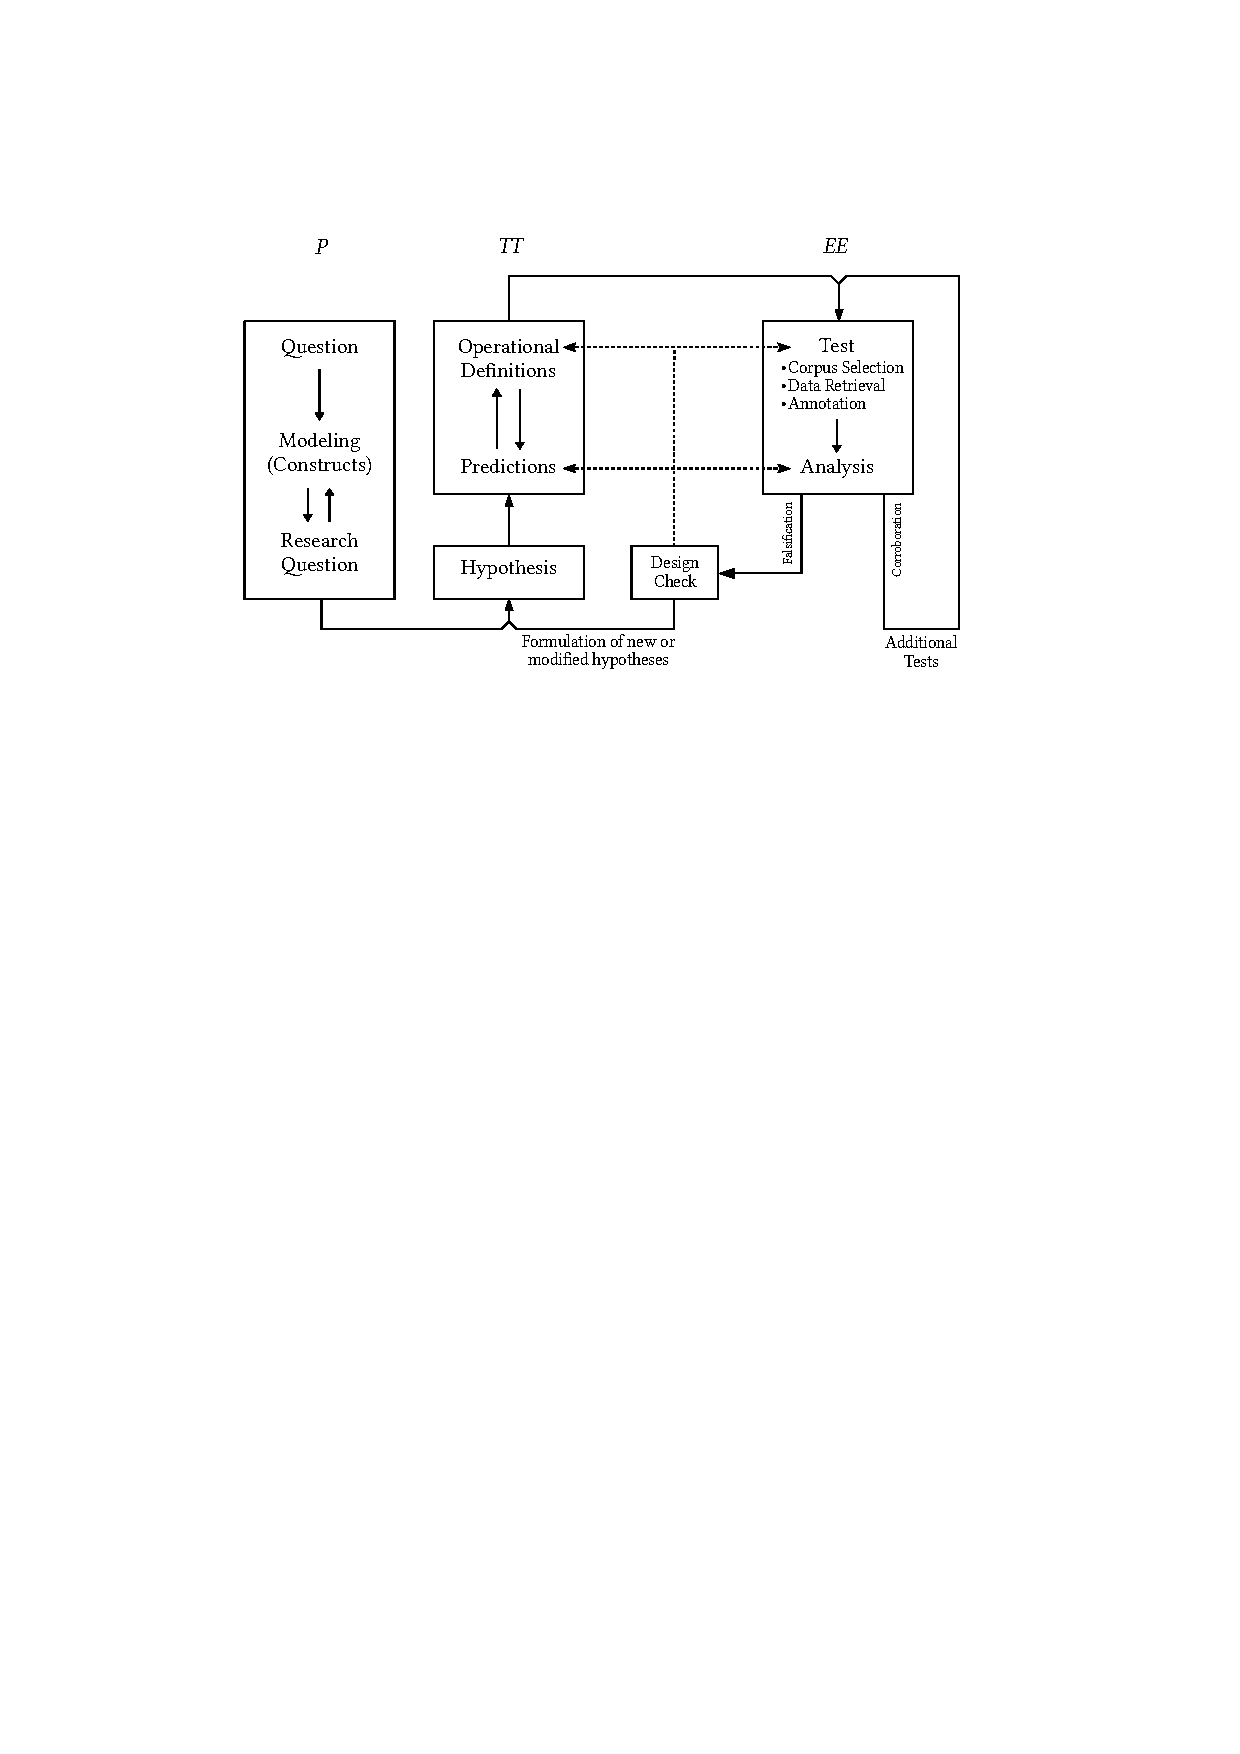
\includegraphics[scale=0.9]{figures/researchcycle}
\end{figure}

Research begins with a general question -- something that intrigues an individual or a group of researchers. The part of reality to which this question pertains is then modeled, i.e., described in terms of theoretical constructs, enabling us to formulate, first, a more specific research question, and often, second, a hypothesis. \is{hypothesis} There is nothing automatic about these steps -- they are typically characterized by lengthy critical discussion, false starts or wild speculation, until testable hypotheses emerge (in some disciplines, this stage has not yet been, and in some cases probably never will be reached). Next, predictions must be derived, requiring operational \is{operationalization} definitions of the constructs posited previously. This may require some back and forth between formulating predictions and providing sufficiently precise operationalizations.

Next, the predictions must be tested -- in the case of corpus linguistics, corpora must be selected and data must be retrieved \is{retrieval} and annotated, \is{annotation} something we will discuss in detail in the next chapter. Then the data are analyzed with respect to the hypothesis. \is{hypothesis} If they corroborate \is{corroboration} the hypothesis (or at least fail to falsify \is{falsification} it), this is not the end of the process: with Popper, we should only begin to accept evidence as corroborating when it emerges from repeated attempts to falsify the hypothesis. Thus, additional tests must be, and typically are, devised. If the results of any test falsify \is{falsification} the hypothesis, this does not, of course, lead to its immediate rejection. After all, we have typically arrived at our hypothesis based on good arguments, and so researchers will typically perform what we could call a ``design \is{research design} check'' on their experiment, \is{experimental method} looking closely at their predictions to see if they really follow from the hypothesis, \is{hypothesis} the operational \is{operationalization} definitions to see whether they are reliable \is{reliability} and valid \is{validity} with respect to the constructs they represent, and the test itself to determine whether there are errors or confounding variables in the data selection and analysis. If potential problems are found, they will be fixed and the test will be repeated. Only if it fails repeatedly will researchers abandon (or modify) the hypothesis.

The repeated testing, and especially the modification of a hypothesis \is{hypothesis} is inherently dangerous, as we might be so attached to our hypothesis that we will keep testing it long after we should have given it up, or that we will try to save it by changing it just enough that our test will no longer falsify \is{falsification} it, or by making it completely untestable \citep[cf.][37]{popper_conjectures_1963}. This must, of course, be avoided, but so must throwing out a hypothesis, \is{hypothesis} or an entire model, on the basis of a single falsification \is{falsification} event. Occasionally, especially in half\hyp{}mature disciplines like linguistics, models morph into competing schools of thought, each vigorously defended by its adherents even in the face of a growing number of phenomena that they fail to account for. In such cases, a radical break in the research cycles within these models may be necessary to make any headway at all -- a so\hyp{}called ``paradigm shifts'' occurs. This means that researchers abandon the current model wholesale and start from scratch based on different initial assumptions \citep[see][]{kuhn_structure_1962}. Corpus linguistics with its explicit recognition that generalizations about the language system can and must be deduced from language usage may present such a paradigm shift with respect to the intuition\hyp{}driven \is{intuition} generative \is{generative linguistics} models.

Finally, note that the scientific research cycle is not only incremental, with each new hypothesis \is{hypothesis} and each new test building on previous research, but that it is also collaborative, with one researcher or group of researchers picking up where another left off. This collaborative nature of research requires researchers to be maximally transparent with respect to their research designs, \is{research design} laying open their data and methods in sufficient detail for other researchers to understand exactly what prediction was tested, how the constructs in question were operationalized, \is{operationalization} how data were retrieved \is{retrieval} and analyzed. Again, this is the norm in disciplines like experimental \is{experimental method} physics and psychology, \is{psychology} but not so much so in the more humanities\hyp{}leaning \is{humanities} disciplines, which tend to put the focus on ideas and arguments rather than methods. We will deal with data retrieval and annotation \is{annotation} in the next chapter and return to the issue of methodological transparency at the end of it.